
\section{Support d'étude \label{ccs_mp_2022_sec_1}}
%I.A - 
\subsection{Contexte \label{ccs_mp_2022_sec_1A}}
\ifprof
\else
L'obligation réglementaire de présence d'appui-têtes dans les voitures a contribué à une meilleure protection des conducteurs et des passagers en limitant les traumatismes dus au «coup du lapin » (figure \ref{ccs_mp_2022_fig_01}). Ce phénomène correspond à un mouvement brusque de flexion-extension de la tête par rapport au buste. Il peut être causé en voiture, lors de chocs à basse vitesse par exemple, ou dans des situations d'embouteillage. Aucune lésion n'est visible en imagerie médicale, cependant les victimes de ce traumatisme cervical souffrent de douleurs handicapantes sur le long terme.\\

\begin{figure}[!h]
\centering
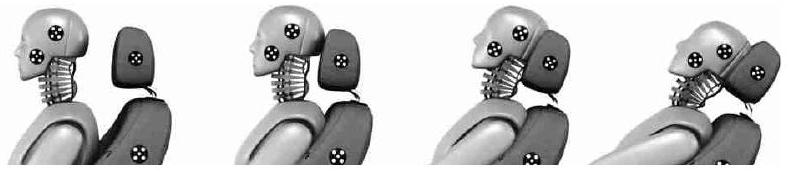
\includegraphics[width=\textwidth]{2025_07_06_ec63d2f3afc18cdeeb83g-01}

%Figure 1 
\caption{Réduction du phénomène du «coup du lapin » par l'usage d'un appui-tête (Référence : R.T. Shone) \label{ccs_mp_2022_fig_01}}
\end{figure}

Les crash-tests automobiles réalisés actuellement, sont effectués, entre autres, grâce à des mannequins de choc instrumentés représentatifs de différentes catégories de morphologie (par exemple, le mannequin représentant $50 \%$ des tests, correspond à un homme mesurant $1,75 \mathrm{~m}$ et pesant 80 kg ). L'étude de la diversité morphologique n'est cependant pas complète. De plus, la contribution musculaire de l'humain qui réagit au choc ne peut pas être étudiée. Mais surtout, les systèmes expérimentaux de crash-tests déjà disponibles ne sont pas représentatifs du phénomène de «coup du lapin» en termes d'accélérations et d'énergie dissipée lors du choc.\\
L'étude proposée porte sur la conception d'un dispositif expérimental, appelé Sled, ainsi que son modèle numérique, qui serviront, dans le cadre de travaux de recherche, à mieux comprendre les phénomènes liés au «coup du lapin » et ainsi à adapter à terme les moyens de prévention et de protection des individus en fonction des morphologies. La conception s'articule en 3 étapes.

\begin{itemize}
  \item Première étape : conception d'un Sled $0,3 g$
\end{itemize}

Afin de comprendre les traumatismes causés par le phénomène de «coup du lapin », il est nécessaire, de développer un dispositif expérimental particulier, permettant de générer des niveaux d'énergie faibles et non lésionnels à un volontaire. Ces faibles niveaux d'énergie correspondent à des accélérations et décélérations fixées à $\pm 0,3 g$ pendant une durée de 1 seconde chacune.

\begin{itemize}
  \item Deuxième étape : élaboration de modèles
\end{itemize}

Ces données, recueillies sur des personnes volontaires, serviront à enrichir une base de données et permettront de développer des modèles de comportement à ce niveau d'énergie, mais aussi à des niveaux d'énergie réels (accélération/décélération de $\pm 1 g$ pendant 1 seconde).

\begin{itemize}
  \item Troisième étape : conception d'un Sled $1 g$
\end{itemize}

Un second dispositif expérimental sera ensuite construit. Avec des accélérations de $\pm 1 g$, les expérimentations ne pourront être conduites qu'avec des mannequins de chocs. Ce second dispositif, plus représentatif en ce qui concerne les niveaux d'accélération, servira alors à affiner les modélisations numériques.

La modélisation biomécanique des individus ainsi que les réactions musculaires des volontaires ne seront pas étudiées ici. Le sujet portera exclusivement sur les deux premières étapes.
Le principe retenu par les ingénieurs du bureau d'études pour concevoir le Sled (figure \ref{ccs_mp_2022_fig_02}) est inspiré des crashtests réalisés dans le domaine automobile :

\begin{itemize}
  \item une plateforme est animée d'un mouvement de translation horizontale par rapport au bâti ;
  \item un passager (volontaire ou mannequin) peut prendre place sur cette plateforme via un siège ;
  \item un dispositif de mise en mouvement permet d'atteindre les accélérations et décélérations attendues.
\end{itemize}


\begin{figure}[!h]
\centering
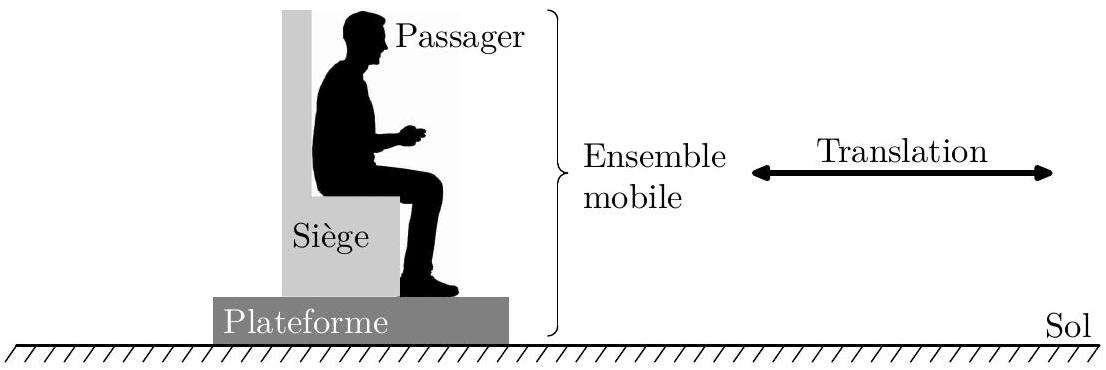
\includegraphics[width=\textwidth]{2025_07_06_ec63d2f3afc18cdeeb83g-02(1)}

%Figure 2 
\caption{Principe retenu pour la conception du Sled \label{ccs_mp_2022_fig_02}}
\end{figure}
\fi

%I.B - 
\subsection{Diagramme partiel des exigences du Sled pour les versions $0,3 g$ et $1 g$ \label{ccs_mp_2022_sec_1B}}
\ifprof
\else
Afin que les accélérations et les vitesses générées soient représentatives du phénomène de "coup du lapin », le Sled doit satisfaire les exigences définies figure \ref{ccs_mp_2022_fig_A} du document réponse.
\fi

%II 
\section{Pré-dimensionnement du Sled $0,3 g$ \label{ccs_mp_2022_sec_2}}
\ifprof
\else
La première étape du développement du Sled $0,3 g$ qui sera utilisé avec des personnes volontaires consiste à prédimensionner certains éléments technologiques pour atteindre les performances définies dans le diagramme des exigences (figure \ref{ccs_mp_2022_fig_A}).

Ainsi, dans une première approche simplifiée, l'ensemble mobile est modélisé par une masse rigide en liaison glissière par rapport au bâti, comme défini sur la figure \ref{ccs_mp_2022_fig_03}. Pour effectuer des campagnes de tests représentatifs du phénomène de coup du lapin avec des personnes volontaires, le profil d'accélération défini sur la figure \ref{ccs_mp_2022_fig_04} est adopté.

\subsubsection*{Modèle cinématique}
\begin{itemize}
  \item Soit $S_{0}$ le bâti lié au sol.
  \item Soit $S$ l'ensemble mobile \{volontaire + siège + plateforme + capteurs\}, en liaison glissière de direction $\vec{x}_{0}$ avec le bâti $S_{0}$.
\end{itemize}

\begin{figure}[!h]
\centering
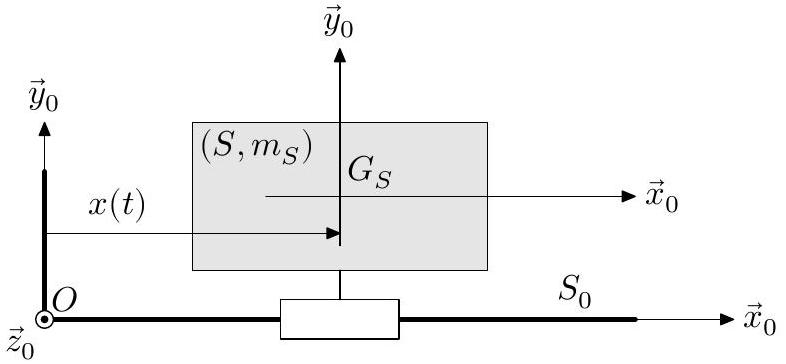
\includegraphics[width=.7\textwidth]{2025_07_06_ec63d2f3afc18cdeeb83g-02}
%Figure 3 
\caption{\label{ccs_mp_2022_fig_03} Modélisation cinématique de l'ensemble mobile $S$ en liaison avec le bâti $S_{0}$}
\end{figure}



\subsubsection*{Notations et données}
\begin{itemize}
  \item Le repère $R_{0}\left(O, \vec{x}_{0}, \vec{y}_{0}, \vec{z}_{0}\right)$ associé au solide $S_{0}$ est supposé galiléen.
  \item Le repère $R_{S}\left(G_{s}, \vec{x}_{0}, \vec{y}_{0}, \vec{z}_{0}\right)$ associé à l'ensemble mobile $S$.
  \item $t$, le temps, exprimé en secondes.
  \item $m_{S}$, la masse de l'ensemble mobile $S, G_{S}$ son centre de gravité tel que $x(t)=\overrightarrow{O G_{S}} \cdot \vec{x}_{0}$.
  \item $\vec{V}_{\left(G_{S}, S / S_{0}\right)}=v(t) \vec{x}_{0}$, la vitesse du centre de gravité $G_{S}$ de l'ensemble mobile $S$ par rapport au bâti $S_{0}$.
  \item $\vec{a}_{\left(G_{S}, S / S_{0}\right)}=a(t) \vec{x}_{0}$, l'accélération du centre de gravité $G_{S}$ de l'ensemble mobile $S$ par rapport au bâti $S_{0}$.
  \item L'accélération de la pesanteur est telle que $\vec{g}=-g \vec{y}_{0}$ avec $g=9,81 \mathrm{~m} \cdot \mathrm{~s}^{-2}$.
\end{itemize}

\subsubsection*{Profil d'accélération type}
\begin{itemize}
  \item L'ensemble mobile $S$ est considéré au repos à l'état initial : ses position, vitesse et accélération sont considérées nulles à l'instant initial.
  \item L'ensemble mobile $S$ est ensuite soumis à un cycle complet d'une accélération constante $a_{c}=+0,3 g$ pendant 1 seconde, puis d'une décélération constante de $-0,3 g$ pendant 1 seconde. Son évolution temporelle, $a(t)$, est présentée sur la figure \ref{ccs_mp_2022_fig_04}.
\end{itemize}

\begin{figure}[!h]
\centering
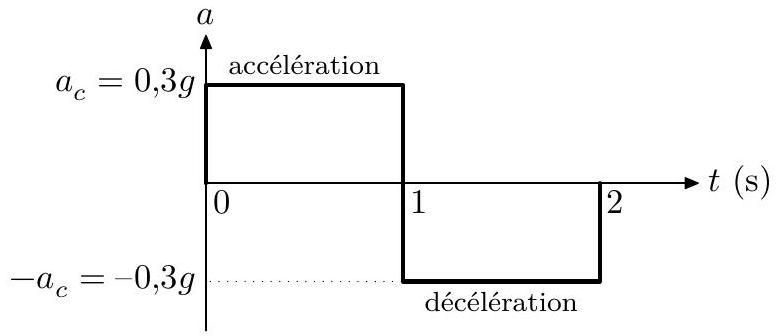
\includegraphics[width=.5\textwidth]{2025_07_06_ec63d2f3afc18cdeeb83g-03}
%Figure 4 
\caption{\label{ccs_mp_2022_fig_04}Évolution de l'accélération au cours du temps}
\end{figure}
%II.A - 
\subsection{Encombrement spatial du Sled 0,3g \label{ccs_mp_2022_sec_2A}}

\begin{obj}
L'objectif est de vérifier que la course du Sled est compatible avec une utilisation dans une salle d'expérimentation.
\end{obj}
\fi


%Q 1. 
\question{\label{ccs_mp_2022_sec_q_01}Déterminer l'expression littérale de la vitesse $v(t)$ en fonction de l'accélération $a_{c}$, dans la première phase d'accélération.}
\ifprof
\begin{corrige}
Lors de la première phase d'accélération on a : $ \dfrac{\text{d}v(t)}{\text{d}t} = a_c \quad \Leftrightarrow \quad \text{d} v(t) = a_c \text{d}t$

D'où : 
$\int_0^t  \text{d} v(t) $ 
$= \int_0^t a_c \text{d}t $
$ = \left[ v(t) \right]_0^t $
$ = \left[ a_c \times t \right]_0^t $
$ = v(t) - v(0) $
$= a_c \times (t - 0) $

Au final, $v(t)  = a_c \times t$.

\end{corrige}
\else
\fi

%Q 2. 
\question{\label{ccs_mp_2022_sec_q_02}En déduire la valeur maximale, notée $V_{\text {max }}$ et exprimée en $\mathrm{m} \cdot \mathrm{s}^{-1}$, de la vitesse atteinte par l'ensemble mobile $S$ au bout d'une seconde avec une accélération constante de $0,3 g$. Conclure sur le respect de l'exigence $\mathrm{Id}=1.1 .2$.}
\ifprof
\begin{corrige}
La fonction $v(t)$ étant continue et croissante, sa valeur maximale est à la fin de la phase d'accélération, soit : $ V_\text{max} = v(1) = a_c \times 1 = 0.3 g \times 1$.

A.N. : $ V_\text{max} = 0.3 \times 9.81 \times 1 = 2.9 \text{ m.s}^{-1} < 3 \text{ m.s}^{-1} \text{  (exigence \texttt{Id 1.1.2})}$.

Donc l'exigence \texttt{Id 1.1.2} est bien respectée.
\end{corrige}
\else
\fi


Un essai complet comprend une phase d'accélération suivie d'une phase de décélération.

%Q 3. 
\question{\label{ccs_mp_2022_sec_q_03}Déterminer la distance maximale théorique, notée $x_{\text {max }}$ et exprimée en m, parcourue par l'ensemble mobile $S$ au cours d'un essai complet. Vérifier le respect de l'exigence Id = 1.2.}
\ifprof
\begin{corrige}
Lors d'un essai complet, il y a une phase d'accélération qui dure une seconde à $\ddot x = a_c$ et une phase de décélération à $\ddot x = - a_c$. On en déduit alors pour chaque phase, les résultats suivants :\\

\begin{minipage}{.5\textwidth}
	\begin{center}Phase d'accélération $\varphi_1$ : pour $t \in [0;1]$\end{center}
$
\begin{array}{l l}
\ddot x_{\varphi_1} & = a_c = 0.3 g\\
\dot x_{\varphi_1} & = v(t) = 0.3 g \times t \rightarrow v(1) = V_\text{max} = 0.3 g \times 1 \\
x_{\varphi_1}(t) & =  0.3 g \times \dfrac{t^2}{2} + x(0) \rightarrow x(1) = \dfrac{0.3}{2} g
\end{array}
$
\end{minipage}
\begin{minipage}{.5\textwidth}
	\begin{center}Phase de décélération $\varphi_2$  : pour $t \in [1;2]$\end{center}
$
\begin{array}{l l}
\ddot x_{\varphi_2} & = -a_c = -0.3 g\\
\dot x_{\varphi_2} & = -0.3 g \times (t-1) + v(1)\\
x_{\varphi_2}(t) & = -0.3 g \times \dfrac{(t-1)^2}{2} + v(1) \times (t-1) + x(1)
\end{array}
$
\end{minipage}

\vspace{1em}
Finalement on a : $x_\text{max} = x_{\varphi_2}(2) = -\dfrac{0.3}{2} g + 0.3 g \times 1 \times 1 + \dfrac{0.3}{2} g$ et $ x_\text{max} = 0.3 g \times 1 \times 1 $.

A.N. $ x_\text{max} = 2.9 \text{ m} < 4.5 \text{ m} \text{  (exigence \texttt{Id 1.2})}$.

Donc l'exigence \texttt{Id 1.2} est bien respectée.
\end{corrige}
\else
\fi

%II.B - 
\subsection{Dimensionnement spatial de l'ensemble mobile \label{ccs_mp_2022_sec_2B}}
%\section*{Objectif}

\begin{obj}
L'objectif est de vérifier la sécurité des passagers et de valider l'emprise au sol du Sled.

Les ingénieurs du bureau d'études envisagent de réaliser la liaison glissière par interposition d'éléments roulants, afin de réduire les pertes énergétiques dans cette liaison et de diminuer également le phénomène d'arc-boutement. Il est à présent nécessaire de vérifier la sécurité des passagers du Sled en étudiant le possible basculement de l'ensemble mobile lors d'un essai.
\end{obj}

\ifprof
\else
\subsubsection*{Hypothèses d'étude}
\begin{itemize}
  \item Pour cette étude, les ingénieurs du bureau d'études choisissent de modéliser la liaison glissière entre l'ensemble mobile $S$ et le bâti $S_{0}$ dans le plan de symétrie ( $O, \vec{x}_{0}, \vec{y}_{0}$ ) de la figure \ref{ccs_mp_2022_fig_05} par deux contacts ponctuels en $A$ et en $B$, de normale $\vec{y}_{0}$, distants de $L$.
  \item L'étude suivante est menée uniquement en phase d'accélération définie pour un essai avec un passager volontaire.
\end{itemize}

\begin{figure}[!h]
\centering
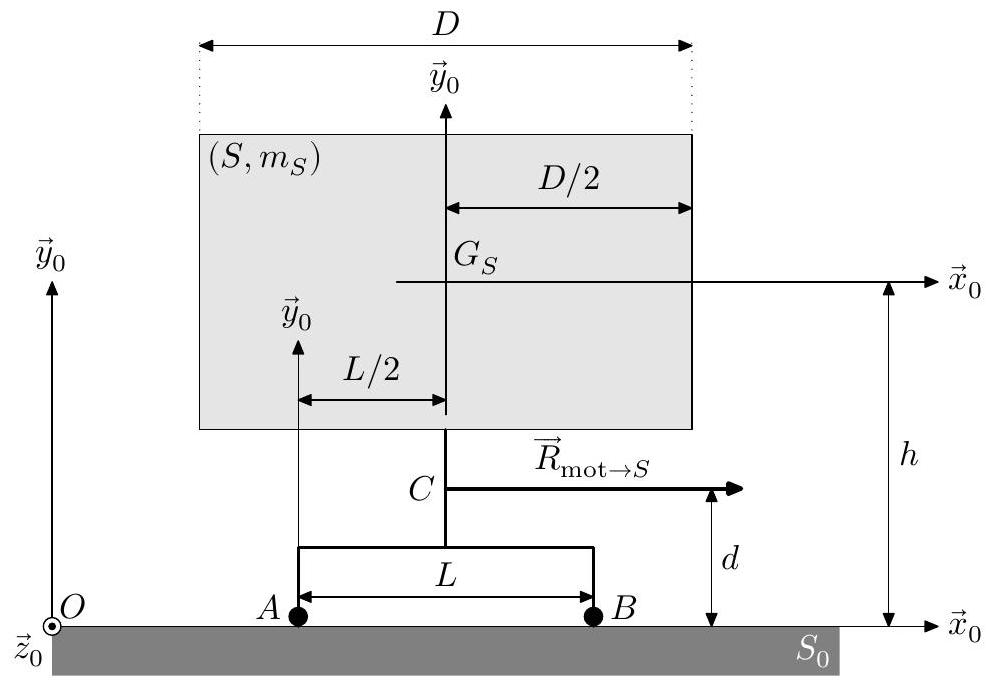
\includegraphics[width=.7\textwidth]{2025_07_06_ec63d2f3afc18cdeeb83g-03(1)}
\caption{\label{ccs_mp_2022_fig_05}Paramétrage de l'ensemble mobile $S$ du Sled}
\end{figure}



\subsubsection*{Notations et données}
\begin{itemize}
  \item Les actions transmissibles par les deux contacts ponctuels seront respectivement notées
\end{itemize}

$$
\left\{T_{A_{S_{0} \rightarrow S}}\right\}=\left\{\begin{array}{c}
Y_{A} \vec{y}_{0} \\
\overrightarrow{0}
\end{array}\right\}_{A} \quad \text { et } \quad\left\{T_{B_{S_{0} \rightarrow S}}\right\}=\left\{\begin{array}{c}
Y_{B} \vec{y}_{0} \\
\overrightarrow{0}
\end{array}\right\}_{B}
$$

\begin{itemize}
  \item L'action mécanique motrice qui permet de mettre en mouvement l'ensemble mobile $S$ par rapport au bâti $S_{0}$ est modélisée par un glisseur au point $C$, noté
\end{itemize}

$$
\left\{T_{\mathrm{mot} \rightarrow S}\right\}=\left\{\begin{array}{c}
\vec{R}_{\mathrm{mot} \rightarrow S}=R \vec{x}_{0} \\
\overrightarrow{0}
\end{array}\right\}_{C}
$$

avec $R>0$ en phase d'accélération.

\begin{itemize}
  \item Les principales caractéristiques dimensionnelles indiquées sur la figure \ref{ccs_mp_2022_fig_05} ont été estimées pour avoir une position réaliste du volontaire dans un siège de voiture, $D=1000 \mathrm{~mm}$, $d=220 \mathrm{~mm}$ et $h=1100 \mathrm{~mm}$.
\end{itemize}
\fi

%II.B.1) 
\subsubsection{Détermination de l'effort normal $Y_{B}$ \label{ccs_mp_2022_sec_2B1}}

%Q 4. 
\question{\label{ccs_mp_2022_sec_q_04}Isoler l'ensemble mobile $S$ et effectuer l'inventaire des actions mécaniques extérieures qui s'appliquent sur cet ensemble.}
\ifprof
\begin{corrige}
On isole $S$, le bilan des actions mécanique à $S$ est :

\begin{itemize}
\item la pesanteur : $\left\{  T_{\text{pes}\to S} \right\} = \begin{Bmatrix} - m_S \, g \, \vec y_0 \\ \overrightarrow{0} \end{Bmatrix}_{G_S}$ 
\item l'action du sol sur $S$ en $A$ : $\left\{  T_{A_{S_0\to S}}\right\} = \begin{Bmatrix} Y_A \, \vec y_0 \\ \overrightarrow{0} \end{Bmatrix}_A $
\item l'action du sol sur $S$ en $B$ :  $\left\{  T_{B_{S_0\to S}}\right\} = \begin{Bmatrix} Y_B \, \vec y_0 \\ \overrightarrow{0} \end{Bmatrix}_B $
\item l'action mécanique motrice : $\left\{ T_{\text{mot}\to S} \right\} = \begin{Bmatrix} \overrightarrow{R}_{\text{mot}\to S} = R \, \vec x_0 \\ \overrightarrow{0} \end{Bmatrix}_C$
\end{itemize}
\end{corrige}
\else
\fi


%Q 5. 
\question{\label{ccs_mp_2022_sec_q_05}Exprimer $\vec{\delta}_{\left(G_{S}, S / S_{0}\right)}$, le moment dynamique en $G_{S}$ de l'ensemble mobile $S$ dans son mouvement par rapport au bâti $S_{0}$. En déduire l'expression littérale du moment dynamique au point $A$ de l'ensemble mobile $S$ dans son mouvement par rapport au bâti $S_{0}$ en fonction de l'accélération $a_{c}$, de la masse $m_{S}$ et d'un paramètre géométrique.}
\ifprof
\begin{corrige}
Le moment dynamique en $G_S$ de l'ensemble $S$ s'exprime comme suit :
$\overrightarrow{\delta}_{G_S, S/S_0} = \left.\dfrac{\text{d} \overrightarrow{\sigma}_{G_S, S/S_0}}{\text{d}t}\right|_{R_0} + m_S \overrightarrow{V}_{G_S} \wedge \overrightarrow{V}_{G_S, S/S_0} = \left.\dfrac{\text{d} \overrightarrow{\sigma}_{G_S, S/S_0}}{\text{d}t}\right|_{R_0} $.

Or :$ \overrightarrow{\sigma}_{G_S, S/S_0} = \overline{\overline{I}}_{G_S, S/S_0} \cdot \overrightarrow{\Omega}_{S/S_0} + m \overrightarrow{G_SG_S} \wedge \overrightarrow{V}_{G_S, S/S_0} = \overline{\overline{I}}_{G_S, S/S_0} \cdot \overrightarrow{\Omega}_{S/S_0}$.

%%La symétrie plane (de plan $(O, \vec x_0, \vec y_0)$) permet de simplifier :
%%
%%\begin{itemize}
%%
%%\item la matrice d'inertie : 
%%$$\overline{\overline{I}}_{G_S, S/S_0} = \begin{pmatrix}  A & -F & {-E}  \\ -F & B & {-D} \\ {-E} & {-D} & C \end{pmatrix}_{G_S, \vec x_0, \vec y_0, \vec z_0}  $$
%%
%%\item le vecteur taux de rotation :
%%$$ \overrightarrow{\Omega}_{S/S_0} = \begin{pmatrix} {\omega_x} \\ {\omega_y} \\ \omega_z \end{pmatrix}_{\vec x_0, \vec y_0, \vec z_0}$$
%%\end{itemize}
%%
%%Le moment cinétique devient alors : $ \overrightarrow{\sigma}_{G_S, S/S_0} = C \, \omega_z \, \vec z_0$
%%
%%Le moment dynamique peut s'écrire : $ \overrightarrow{\delta}_{G_S, S/S_0} = C \dfrac{\text{d}\omega_z}{\text{d}t} \vec z_0$
%
Si on considère qu'on a une liaison glissière de $S/S_0$, alors $\left\{ \mathcal{V}_{S/S_0} \right\} = \begin{Bmatrix} \vec 0 \\ v(t) \vec x_0 \end{Bmatrix}_{G_S}$, donc $\overrightarrow{\Omega}_{S/S_0} = \vec 0$

Donc $\overrightarrow{\sigma}_{G_S, S/S_0} = \vec 0$, d'où :
$ \overrightarrow{\delta}_{G_S, S/S_0} = \vec 0$.


D'après le théorème de Varignon, on a :
$\overrightarrow{\delta}_{A, S/S_0} = \overrightarrow{\delta}_{G_S, S/S_0} + \overrightarrow{AG_S} \wedge m_S \, \overrightarrow{a}_{G_S, S/S_0} $
 $= \vec 0 + \begin{pmatrix}  \dfrac{L}{2} \\ h \\ 0 \end{pmatrix}_{\vec x_0, \vec y_0, \vec z_0} \wedge m_S \begin{pmatrix}  a_c \\ 0 \\ 0 \end{pmatrix}_{\vec x_0, \vec y_0, \vec z_0}$.


Au final, $ \overrightarrow{\delta}_{A, S/S_0} =  - m_S \times h \times a_c \times \vec z_0 $.



\end{corrige}
\else
\fi

%Q 6. 
\question{\label{ccs_mp_2022_sec_q_06}Appliquer le théorème du moment dynamique, à l'ensemble mobile $S$, au point $A$, en projection selon $\vec{z}_{0}$. En déduire l'expression littérale de la composante $Y_{B}$ du contact ponctuel en $B$ en fonction de l'accélération $a_{c}$, de $g$, de la masse $m_{S}$, de paramètres géométriques et de $R$.}
\ifprof
\begin{corrige}
D'après le théorème du moment dynamique appliqué en $A$, en projection sur $\vec z_0$, on a :

$\left( \overrightarrow{\mathcal{M}}_{A, \text{pes} \to S} +  \overrightarrow{\mathcal{M}}_{A, B_{S_0\to S}} + \overrightarrow{\mathcal{M}}_{A, \text{mot} \to S} \right) \cdot \vec z_0 = \overrightarrow{\delta}_{A, S/S_0} \cdot \vec z_0 $.

Il faut donc déplacer les torseurs du bilan des actions mécaniques extérieures en $A$ :

\begin{itemize}
\item $\left\{  T_{\text{pes}\to S} \right\} = \begin{Bmatrix} - m_S \, g \, \vec y_0 \\ \overrightarrow{0} \end{Bmatrix}_{G_S} = \begin{Bmatrix} - m_S \, g \, \vec y_0 \\ \overrightarrow{AG_S} \wedge - m_S \, g \, \vec y_0  = - m_S \times g \times \dfrac{L}{2} \vec z_0 \end{Bmatrix}_{A}  \quad \left(\text{avec : } \overrightarrow{AG_S} = \dfrac{L}{2} \vec x_0 + h \vec y_0 \right)$
\item $\left\{  T_{A_{S_0\to S}}\right\} = \begin{Bmatrix} Y_A \, \vec y_0 \\ \overrightarrow{0} \end{Bmatrix}_A $
\item $\left\{  T_{B_{S_0\to S}}\right\} = \begin{Bmatrix} Y_B \, \vec y_0 \\ \overrightarrow{0} \end{Bmatrix}_B = \begin{Bmatrix} Y_B \, \vec y_0 \\ \overrightarrow{AB} \wedge Y_B \, \vec y_0 = L \times Y_B \vec z_0 \end{Bmatrix}_A \quad \left(\text{avec : } \overrightarrow{AB} = L \vec x_0 \right)$
\item $\left\{ T_{\text{mot}\to S} \right\} = \begin{Bmatrix} R \, \vec x_0 \\ \overrightarrow{0} \end{Bmatrix}_C = \begin{Bmatrix} R \, \vec x_0 \\ \overrightarrow{AC} \wedge R \, \vec x_0 = - d \times R \vec z_0 \end{Bmatrix}_A \quad \left(\text{avec : } \overrightarrow{AC} = \dfrac{L}{2} \vec x_0 + d \vec y_0 \right)$
\end{itemize}

Le théorème du moment dynamique appliqué en $A$ projeté sur $\vec z_0$ s'écrit alors :
$ - m_S \times g \times \dfrac{L}{2} + L \times Y_B - d \times R = - m_S \times h \times a_c $.

Finalement, on obtient l'expression littérale de la composante $Y_B$ :

$ Y_B = \dfrac{m_S \left(g \times \dfrac{L}{2} -\times h \times a_c\right) + d \times R}{L}$
$  = m_S \left( \dfrac{g}{2} - \dfrac{h \times a_c}{L}\right) + \dfrac{d \times R}{L}$.
\end{corrige}
\else
\fi


%II.B.2) 
\subsubsection*{Détermination de la longueur $L$ \label{ccs_mp_2022_sec_2B2}}

%Q 7. 
\question{\label{ccs_mp_2022_sec_q_07}Donner la condition sur $Y_{B}$ qui traduit le non-basculement autour de l'axe ( $A, \vec{z}_{0}$ ) de l'ensemble mobile $S$ lors de la phase d'accélération.}
\ifprof
\begin{corrige}
La condition traduisant le non-basculement est : $ Y_B > 0$.
\end{corrige}
\else
\fi


%Q 8. 
\question{\label{ccs_mp_2022_sec_q_08}Après avoir explicité le système isolé et précisé le théorème utilisé, déterminer l'expression littérale de $R$, en fonction de la masse $m_{S}$ et de l'accélération $a_{c}$.}
\ifprof
\begin{corrige}
On isole l'ensemble mobile $S$ du Sled et on applique le théorème de la résultante dynamique projeté sur l'axe $\vec x_0$ :
$ R = m_S \times \overrightarrow{a}_{G_S, S/S_0} \cdot \vec x_0$ et
$ R = m_S \times a_c$.
\end{corrige}
\else
\fi


%Q 9. 
\question{\label{ccs_mp_2022_sec_q_09}En déduire la longueur minimale du guidage entre l'ensemble mobile $S$ et le bâti $S_{0}$ en fonction de l'accélération $a_{c}$, de $g$ et de paramètres géométriques pour garantir le non-basculement autour de l'axe ( $A, \vec{z}_{0}$ ) lors de la phase d'accélération.}
\ifprof
\begin{corrige}
En prenant en compte la condition de non-basculement et le résultat du théorème de la résultante dynamique appliquée à $S$ en projection sur $\vec x_0$, on obtient :
$  m_S \left( \dfrac{g}{2} - \dfrac{h \times a_c}{L}\right) + \dfrac{d \times m_S \times a_c}{L} > 0$
et $  L > \dfrac{2\,a_c}{g} (h - d)$.

\end{corrige}
\else
\fi


%II.B.3) 
\subsubsection{Validation des exigences associées à la sécurité des passagers et à l'encombrement \label{ccs_mp_2022_sec_2B3}}
%Q 10. 
\question{\label{ccs_mp_2022_sec_q_10}Au regard de l'expression littérale de la longueur minimale du guidage de l'ensemble mobile $S$, indiquer s'il est nécessaire d'adapter cette longueur aux différentes masses de passagers, volontaires ou mannequins.}
\ifprof
\begin{corrige}
La longueur étant indépendante de la masse de l'ensemble isolé $S$, on en déduit qu'il n'est pas nécessaire d'adapter cette longueur $L$ aux différentes masses de passagers, volontaires ou mannequins.
\end{corrige}
\else
\fi


%Q 11. 
\question{\label{ccs_mp_2022_sec_q_11}Déterminer la valeur numérique minimale de la dimension longitudinale $L$ du guidage entre l'ensemble mobile $S$ et le bâti $S_{0}$ afin de garantir le respect de l'exigence Id $=1.3$ lors de la phase d'accélération définie.}
\ifprof
\begin{corrige}
L'exigence \texttt{Id = 1.3} de non-basculement donne que la dimension longitudinale minimale est :
$ L_\text{min} = \dfrac{2\,a_c}{g} (h - d) = \dfrac{2\times 0.3 g}{g} (h - d)$.

A.N. :$ L_\text{min} = 2 \times 0.3 \times (1100 - 220) = 528 \text{ mm}$.
\end{corrige}
\else
\fi


%Q 12. 
\question{\label{ccs_mp_2022_sec_q_12}Conclure quant au respect de l'exigence $\mathrm{Id}=1.2$.}
\ifprof
\begin{corrige}
L'exigence \texttt{Id = 1.2} impose une dimension maximale du Sled de $4.5$ m. 

Or la dimension du Sled est $X+L_\text{min}$ d'où l'application numérique :
$ X + L_\text{min} = 2.9 + 0.528 = 3.428 \text{ m} < 4.5 \text{ m}$. 
L'exigence \texttt{Id = 1.2} est donc bien respectée.
\end{corrige}
\else
\fi

\ifprof
\else

\ifprof
\else
Cette étude a conduit les ingénieurs à concevoir une solution pour la liaison glissière mettant en œuvre des galets positionnés au-dessus et en dessous d'un rail (figure \ref{ccs_mp_2022_fig_06}). Des systèmes de réglages sont prévus pour garantir le contact bilatéral et ainsi réduire le risque possible de basculement de l'ensemble mobile $S$.\\
\fi

\begin{figure}[!h]
\centering
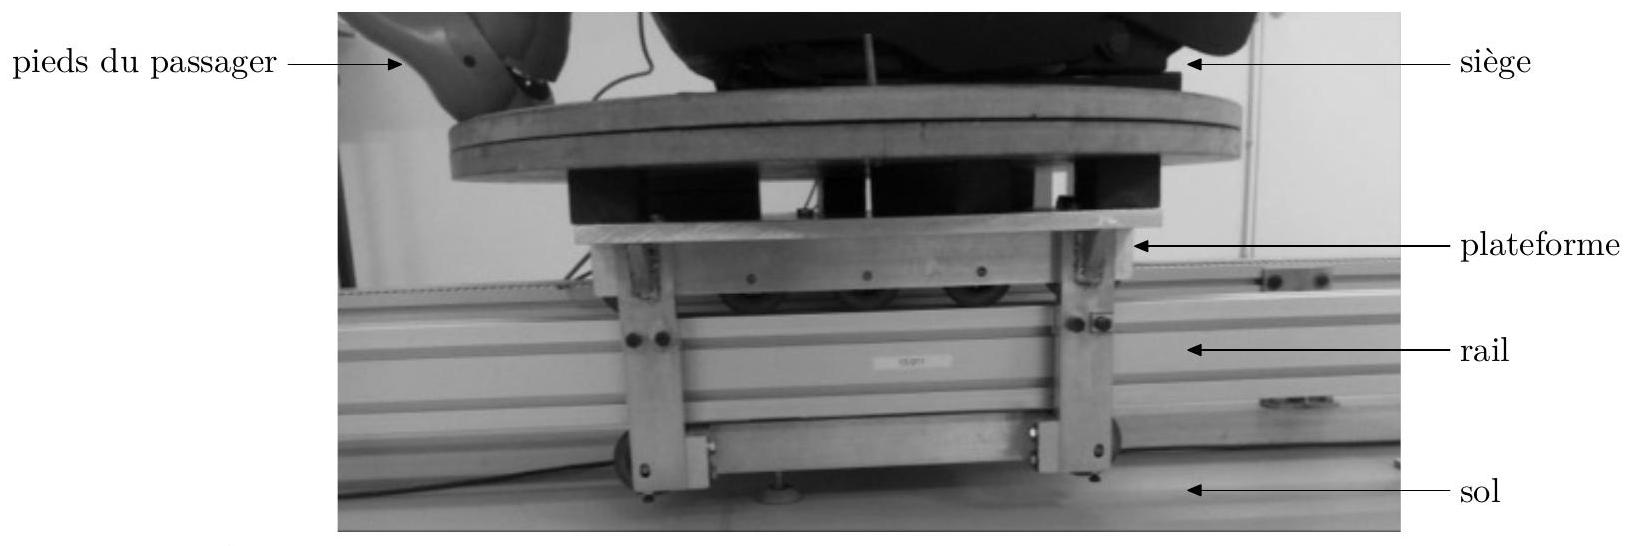
\includegraphics[width=\textwidth]{2025_07_06_ec63d2f3afc18cdeeb83g-04}

%Figure 6 
\caption{\label{ccs_mp_2022_fig_06}Solution retenue pour la réalisation de la liaison glissière entre l'ensemble mobile et le bâti}
\end{figure}
\fi

%III 
\section{Mise en place d'un modèle numérique pour le Sled $0,3 g$ \label{ccs_mp_2022_sec_3}}

\ifprof
\else
Le bureau d'études décide de poursuivre le dimensionnement en modélisant l'asservissement du Sled. Il sera ainsi possible de définir la structure de commande de l'actionneur qui permettra de respecter les exigences définies dans le diagramme présenté en figure \ref{ccs_mp_2022_fig_A}.
\fi

%III.A -
\subsection{Commande en vitesse sans correction \label{ccs_mp_2022_sec_3A}}
\begin{obj}
L'objectif consiste dans un premier temps à valider, à partir d'un modèle, le principe d'une structure d'asservissement en vitesse, sur une commande en accélération.
\end{obj}

\ifprof
\else
Un premier modèle multiphysique (modèle $\mathrm{n}^{\circ} 1$, figure \ref{ccs_mp_2022_fig_20}) a été réalisé par les ingénieurs du bureau d'études à partir des éléments fournis par le prédimensionnement réalisé précédemment.

\subsubsection*{Hypothèses d'étude}
Le modèle proposé comporte trois parties :
\begin{itemize}
  \item une partie électrique avec un moteur contrôlé en courant qui convertit l'énergie électrique en énergie mécanique en rotation ;
  \item une partie mécanique en rotation constituée d'un axe moteur et de ses frottements internes ;
  \item une partie mécanique en translation issue d'un dispositif de transformation de mouvement de rotation en mouvement de translation. Le dispositif associé de type pignon-crémaillère est considéré parfaitement rigide. Cette partie mécanique en translation comporte les différentes masses embarquées : plateforme + siège + capteurs et volontaire.
\end{itemize}

La particularité de ce modèle réside dans le fait qu'il s'agit d'une structure d'asservissement en vitesse, sur une commande en accélération. En effet, afin de répondre à la problématique exposée en introduction, la consigne appliquée au modèle est une accélération de $+0,3 g$ appliquée pendant une durée de 1 seconde, suivi d'une accélération de $-0,3 g$ (ou décélération) appliquée pendant une durée de 1 seconde également (figure \ref{ccs_mp_2022_fig_04}).

Les performances attendues (stabilité, précision, rapidité...) et définies dans le diagramme des exigences (figure \ref{ccs_mp_2022_fig_A}) sont donc des performances en accélération (sauf indication contraire). Cette consigne en accélération est adaptée pour permettre la commande en vitesse du moteur. Un asservissement en vitesse est réalisé à l'aide d'un capteur de vitesse de gain unitaire.
\fi

%Q 13. 
\question{\label{ccs_mp_2022_sec_q_13}Quels sont les rôles respectifs des blocs A et B du modèle $\mathrm{n}^{\circ} 1$ (figure \ref{ccs_mp_2022_fig_20}) ?}
\ifprof
\begin{corrige}
Le bloc A est un intégrateur : $A(p) = \dfrac{1}{p}$.
Le bloc B est un dérivateur : $B(p) = p$.
\end{corrige}
\else
\fi

\ifprof
\else
La modélisation multiphysique proposée peut ainsi être modélisée sous la forme d'un schéma bloc (figure \ref{ccs_mp_2022_fig_07}).

\begin{figure}[!h]
\centering
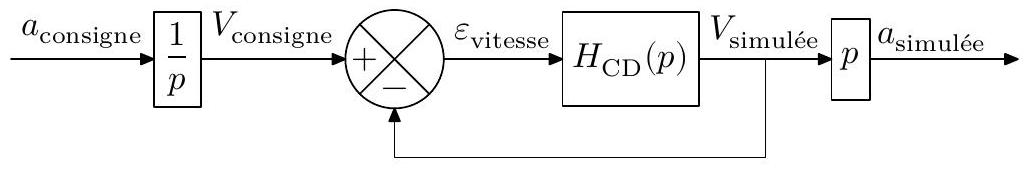
\includegraphics[width=.7\textwidth]{2025_07_06_ec63d2f3afc18cdeeb83g-05}
%Figure 7
\caption{\label{ccs_mp_2022_fig_07}Modélisation $\mathrm{n}^{\circ} 1$ du Sled sous forme de schéma bloc à retour unitaire}
\end{figure}




\subsubsection*{Notations et données}
\begin{itemize}
  \item L'ensemble des trois parties du modèle décrites précédemment (électrique, mécanique en rotation et mécanique en translation) constitue la chaine directe du système que l'on modélise par la fonction de transfert $H_{\mathrm{CD}}(p)$.
  \item La fonction de transfert de l'asservissement en accélération est modélisée sous la forme
\end{itemize}

$$
H_{\mathrm{acc}}(p)=\frac{\text { Accélération simulée }(p)}{\text { Consigne accélération }(p)}=\frac{a_{\text {simulée }}(p)}{a_{\text {consigne }}(p)} .
$$

\begin{itemize}
  \item La fonction de transfert de l'asservissement en vitesse en boucle ouverte peut s'écrire sous la forme d'un second ordre :
\end{itemize}

$$
H_{\mathrm{BO}}(p)=H_{\mathrm{CD}}(p)=\frac{\text{Vitesse simulee}(p)}{\text{Ecart vitesse}(p)}=\frac{V_{\text {simulée }}(p)}{\varepsilon_{\text {vitesse }}(p)}=\frac{K_{\mathrm{BO}}}{1+\frac{2 \xi_{\mathrm{BO}}}{\omega_{0_{\mathrm{BO}}}} p+\frac{1}{\omega_{0_{\mathrm{BO}}}^{2}} p^{2}} .
$$

\begin{itemize}
  \item La fonction de transfert de l'asservissement en vitesse en boucle fermée est modélisée sous la forme :
\end{itemize}

$$
H_{\mathrm{BF}}(p)=\frac{\text { Vitesse simulée }(p)}{\text { Consigne vitesse }(p)}=\frac{V_{\text {simulée }}(p)}{V_{\text {consigne }}(p)} .
$$

\begin{itemize}
  \item Il est rappelé que pour la pulsation de résonance, notée $\omega_{r}$, le gain en décibel s'exprime sous la forme :
\end{itemize}

$$
G_{\mathrm{dB}-\mathrm{BO}}\left(\omega=\omega_{r}\right)=20 \log \left(\frac{K_{\mathrm{BO}}}{2 \xi_{\mathrm{BO}} \sqrt{1-\xi_{\mathrm{BO}}^{2}}}\right)
$$

Pour effectuer la commande en accélération du modèle $\mathrm{n}^{\circ} 1$ (figure \ref{ccs_mp_2022_fig_20}), les ingénieurs du bureau d'études proposent de travailler sur la commande en vitesse.
\fi

%Q 14. 
\question{\label{ccs_mp_2022_sec_q_14}Justifier cette proposition en déterminant la fonction de transfert en accélération $H_{\text {acc }}(p)$ en fonction de $H_{\mathrm{BF}}(p)$. Conclure sur l'intérêt de cette proposition.}
\ifprof
\begin{corrige}
$$H_\text{acc}(p) = \dfrac{1}{{p}} \times H_\text{BF}(p) \times {p} = H_\text{BF}(p)$$

L'intérêt de cette proposition est de pouvoir contrôler le système en vitesse, à l'aide d'une mesure d'accélération (plus simple à implémenter sur le système à l'aide d'un accéléromètre qui fournit directement l'accélération du solide $S$.
\end{corrige}
\else
\fi

\ifprof
\else
Une première simulation avec ce modèle $\mathrm{n}^{\circ} 1$ (figure \ref{ccs_mp_2022_fig_20}) permet d'obtenir le diagramme de Bode de l'asservissement en vitesse en boucle ouverte $H_{\mathrm{BO}}(p)$, proposé en figure \ref{ccs_mp_2022_fig_08} .

\begin{figure}[!h]
\centering
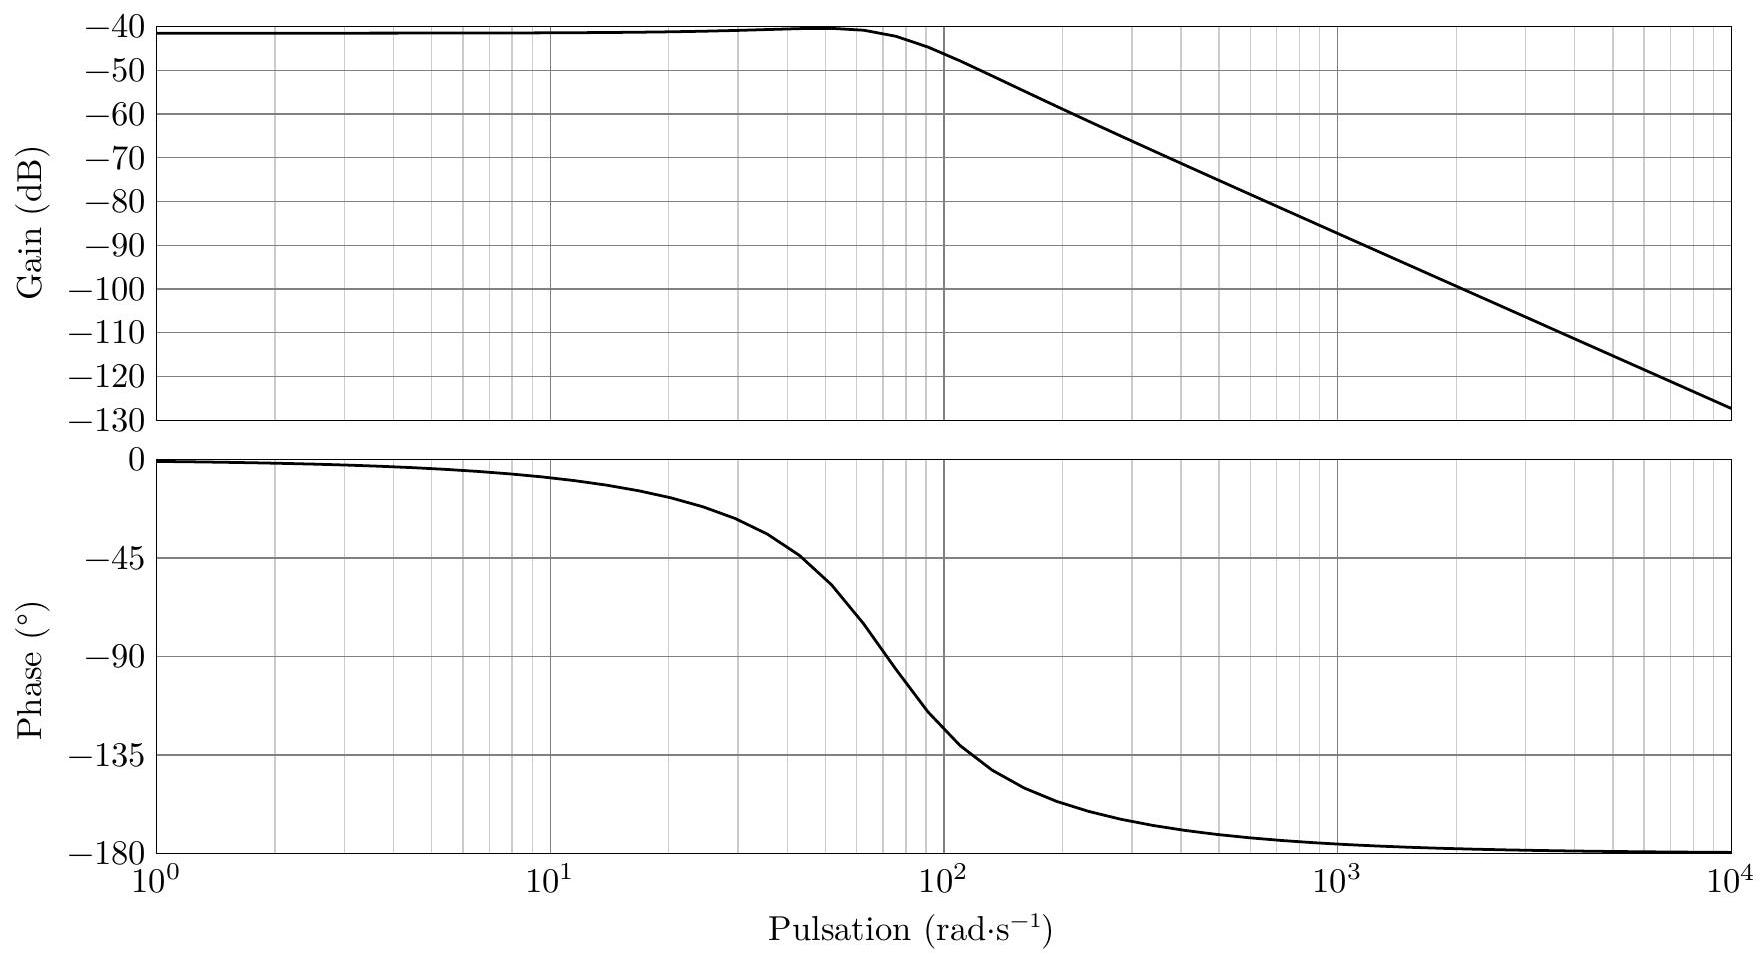
\includegraphics[width=\textwidth]{2025_07_06_ec63d2f3afc18cdeeb83g-06}
%Figure 8 
\caption{\label{ccs_mp_2022_fig_08}Diagramme de Bode en boucle ouverte de l'asservissement en vitesse du modèle $\mathrm{n}^{\circ} 1$ (figure \ref{ccs_mp_2022_fig_20})}
\end{figure}
\fi


%Q 15. 
\question{\label{ccs_mp_2022_sec_q_15}Évaluer graphiquement les marges de stabilité du système et conclure sur le respect de l'exigence Id =1.1.1.1.1.}
\ifprof
\begin{corrige}
L'exigence \texttt{Id = 1.1.1.1.1} requiert une marge de gain $M_\text{gain} > 7$ dB et une marge de phase $M_\varphi > 30$°.

En \textsc{Figure} \ref{fig:sled8}, on remarque que le gain n'est jamais positif ou nul, la marge de phase est donc infinie (ou n'existe pas). De même, la phase n'atteint jamais la valeur de $-180$°, on peut observer une asymptote, la marge de gain est donc infinie (ou n'existe pas).

L'exigence \texttt{Id = 1.1.1.1.1} est donc respectée. 
\end{corrige}
\else
\fi


Une résonance de $+1,1 \mathrm{~dB}$ par rapport à l'asymptote horizontale située à $-41,5 \mathrm{~dB}$ est observée à la pulsation de $49,4 \mathrm{rad} \cdot \mathrm{s}^{-1}$.

%Q 16. 
\question{\label{ccs_mp_2022_sec_q_16}Calculer les valeurs numériques des paramètres $K_{\mathrm{BO}}, \omega_{0_{\mathrm{BO}}}$ et $\xi_{\mathrm{BO}}$ de la fonction de transfert en boucle ouverte $H_{\mathrm{BO}}(p)$ de l'asservissement en vitesse.}
\ifprof
\begin{corrige}
\begin{description}
\item[$K_\text{BO}$] : si l'asymptote horizontale est située à $-41.5$ dB, alors on a
$$ 20\text{log}_{10} (K_\text{BO}) = -41.5 \Leftrightarrow K_\text{BO} = 10^{-41.5/20} = 8.41 \times 10^{-3}$$

\item[$\xi_\text{BO}$] : le gain en décibel lors de la pulsation de résonance permet de déterminer la valeur du facteur d'amortissement. On a $20 \text{log}_{10} \left( \left| H_\text{BO}(j \omega_\text{reson.}) \right| \right)= 20 \text{log}_{10} \left( \dfrac{K_\text{BO}}{\sqrt{\left(  1 - \left( \dfrac{\omega_\text{reson.}}{\omega_{0_\text{BO}}} \right)^2\right)^2 +  \left(\dfrac{2 \xi_\text{BO} \omega_\text{reson.}}{\omega_{0_\text{BO}}}\right)^2} }\right)$

d'après la relation de la pulsation de résonance $\omega_\text{reson.} = \omega_{0_{BO}} \times \sqrt{1 - 2 \xi_\text{BO}^2}$, on obtient le gain en décibel suivant :

$\begin{array}{ll}
20 \text{log}_{10} \left( \left| H_\text{BO}(j \omega_\text{reson.}) \right| \right) &= 20 \text{log}_{10} \left( \dfrac{K_\text{BO}}{\sqrt{\left(  1 - \sqrt{1 - 2 \xi_\text{BO}^2}\right)^2 +  \left(2 \xi_\text{BO} \sqrt{1 - 2 \xi_\text{BO}^2}\right)^2} }\right)\\
 & = 20 \text{log}_{10} (K_\text{BO}) - 20 \text{log}_{10}\left( 2\xi_\text{BO} \sqrt{1 - \xi_\text{BO}^2}\right)\\
\end{array}
$

d'où :

\begin{minipage}{.35\textwidth}
\def\arraystretch{2}
$\begin{array}{ll}
&- 20 \text{log}_{10}\left( 2\xi_\text{BO} \sqrt{1 - \xi_\text{BO}^2}\right) = 1.1\\
\Leftrightarrow & 2 \xi_\text{BO} \sqrt{1 - \xi_\text{BO}^2} = 10^{-1.1/20}\\
\Leftrightarrow & 4 \xi_\text{BO}^2 \left(1 - \xi_\text{BO}^2\right) = 10^{-2.2/20}\\
\Leftrightarrow & 4 \xi_\text{BO}^2 - 4 \xi_\text{BO}^4 = 10^{-2.2/20}\\
\Leftrightarrow & 4 \xi_\text{BO}^4 - 4 \xi_\text{BO}^2 + 10^{-2.2/20} = 0\\
%\Leftrightarrow & 4 \xi_\text{BO}^2 - 4 \xi_\text{BO}^4 = 10^{-2.2/20}\\
\end{array}
$
\end{minipage}
\begin{minipage}{.65\textwidth}
\def\arraystretch{2}
$\begin{array}{l}
\Delta = (-4)^2 - 4 \times 4 \times 10^{-2.2/20} \simeq 3.6\\
\xi_\text{BO}^2 = \dfrac{-(-4)\pm\sqrt{\Delta}}{2 \times 4} = \{0.737; 0.263\} \\
\xi_\text{BO} = \{0.859; 0.513\}  \text{\quad (car $\xi_\text{BO}$ est défini positivement)}\\
\xi_\text{BO} = 0.513  \text{\quad (car la résonance impose $\xi_\text{BO} < \sqrt{2}/2 \simeq 0.707$)}
\end{array}
$
\end{minipage}


\item[$\omega_{0_\text{BO}}$] : on a simplement $ \omega_{0_\text{BO}} = \dfrac{\omega_\text{reson.}}{\sqrt{1 - 2 \xi_\text{BO}^2}}$
A.N. :
$ \omega_{0_\text{BO}} = \dfrac{49.4}{\displaystyle\sqrt{1 - 2 \times 0.513^2}} \simeq 71.8 \text{ rad.s}^{-1}$.
\end{description}
\end{corrige}
\else
\fi


%Q 17. 
\question{\label{ccs_mp_2022_sec_q_17}Déterminer la fonction de transfert en boucle fermée $H_{\mathrm{BF}}(p)$ en fonction de $K_{\mathrm{BO}}, \omega_{0_{\mathrm{BO}}}$ et $\xi_{\mathrm{BO}}$. Identifier ses coefficients $K_{\mathrm{BF}}, \omega_{0_{\mathrm{BF}}}$ et $\xi_{\mathrm{BF}}$ en fonction de $K_{\mathrm{BO}}, \omega_{0_{\mathrm{BO}}}$ et $\xi_{\mathrm{BO}}$.}
\ifprof
\begin{corrige}
D'après la \textsc{Figure} \ref{fig:sled7} et la formule de Black, on obtient l'expression de la fonction de transfert en boucle fermée suivante :

$H_\text{BF}(p)  = \dfrac{H_\text{BO}(p)}{1 + H_\text{BO}(p)}$
 $ = \dfrac{\dfrac{K_\text{BO}}{1+\dfrac{2 \xi_\text{BO}}{\omega_{0_\text{BO}}}p + \dfrac{1}{\omega^2_{0_\text{BO}}}p^2} }{1 + \dfrac{K_\text{BO}}{1+\dfrac{2 \xi_\text{BO}}{\omega_{0_\text{BO}}}p + \dfrac{1}{\omega^2_{0_\text{BO}}}p^2} }$.
$H_\text{BF}(p)   = \dfrac{\dfrac{K_\text{BO}}{1+K_\text{BO}}}{ 1 + \dfrac{2 \xi_\text{BO}}{\omega_{0_\text{BO}} (1 + K_\text{BO})}p + \dfrac{1}{\omega^2_{0_\text{BO}}(1 + K_\text{BO})}p^2}$

d'où l'identification suivante :
$
\left\{  
\begin{array}{ll}
K_\text{BF} &= \dfrac{K_\text{BO}}{1+K_\text{BO}} \\
\omega_{0_{\text{BF}}} &= \omega_{0_\text{BO}} \sqrt{(1 + K_\text{BO})} \\
\xi_\text{BF} &= \dfrac{\xi_\text{BO}}{\sqrt{1 + K_\text{BO}}}\\
\end{array}
\right.
$


\end{corrige}
\else
\fi

\ifprof
\else
La suite du questionnement sera effectuée avec les valeurs numériques suivantes:

$$
K_{\mathrm{BO}}=8,4 \times 10^{-3}, \quad \xi_{\mathrm{BO}}=0,5, \quad K_{\mathrm{BF}}=8,3 \times 10^{-3}, \quad \omega_{0_{\mathrm{BF}}}=71,9 \mathrm{rad} \cdot \mathrm{~s}^{-1}, \quad \xi_{\mathrm{BF}}=0,5 .
$$

L'abaque du premier dépassement relatif en fonction du facteur d'amortissement est donné en figure \ref{ccs_mp_2022_fig_09}.
\fi

%Q 18. 
\question{\label{ccs_mp_2022_sec_q_18}Déterminer la valeur en $\%$ du premier dépassement et conclure au regard de l'exigence $\mathrm{Id}=1.1 .1 .1 .2$.}
\ifprof
\begin{corrige}
Connaissant le facteur d'amortissement en boucle fermé $\xi_\text{BF} = 0.5$, on peut lire en \textsc{Figure} \ref{fig:sled9} un dépassement de $0.16$ soit $16\%$ environ.

L'exigence \texttt{Id = 1.1.1.1.2} avec un dépassement qui doit être inférieur à $20\%$ est donc bien respectée.

\end{corrige}
\else
\fi


%Q 19. 
\question{\label{ccs_mp_2022_sec_q_19}Déterminer l'expression de l'erreur d'accélération en régime permanent $\varepsilon_{a}$ suite à une entrée de type échelon en accélération d'amplitude $0,3 g$ en fonction de $K_{\mathrm{BO}}$. Faire l'application numérique.}
\ifprof
\begin{corrige}
L'erreur d'accélération (à ne pas confondre avec l'écart) est défini comme suit :

$ \varepsilon_\text{acc} = \lim\limits_{t \to \infty} a_\text{consigne}(t) - a_\text{simulé}(t)$
 $= \lim\limits_{p \to 0} p \times \left(  a_\text{consigne}(p) - a_\text{simulé}(p)\right)$
 d'après le théorème de la valeur finale.

$ \varepsilon_\text{acc}= \lim\limits_{p \to 0} p \times \left( p V_\text{consigne}(p) - p V_\text{simulée}(p) \right)$
 $= \lim\limits_{p \to 0} p \times p V_\text{consigne}(p) \left( 1 - H_\text{BF}(p) \right)$
 $= \lim\limits_{p \to 0} p \times a_\text{consigne}(p) \left( 1 - H_\text{BF}(p) \right)$
 $= \lim\limits_{p \to 0} {p} \times \dfrac{0.3 g}{{p}} \left( 1 - \dfrac{\dfrac{K_\text{BO}}{1+K_\text{BO}}}{ 1 + \dfrac{2 \xi_\text{BO}}{\omega_{0_\text{BO}} (1 + K_\text{BO})}p + \dfrac{1}{\omega^2_{0_\text{BO}}(1 + K_\text{BO})}p^2} \right)$
  $= 0.3 g\left( 1 -\dfrac{K_\text{BO}}{1+K_\text{BO}} \right)$

Au final, $\varepsilon_\text{acc} =  \dfrac{0.3 g}{1+K_\text{BO}} $.

A.N. : $ \varepsilon_\text{acc} = \dfrac{0.3 \times 9.81}{1 + 8.4 \times 10^{-3}} \simeq 2.918 \text{ m.s$^{-2}$}$.

\end{corrige}
\else
\fi


%Q 20. 
\question{\label{ccs_mp_2022_sec_q_20}En déduire l'erreur relative en $\%$ et conclure sur l'exigence $\mathrm{Id}=1.1 .1 .2 .1$.}
\ifprof
\begin{corrige}
L'erreur relative vaut :

$ \varepsilon_\text{relatif} = \lim\limits_{t \to \infty}\dfrac{a_\text{consigne}(t) - a_\text{simulé}(t)}{a_\text{consigne}(t)}$
 $= \dfrac{\varepsilon_\text{acc}}{0.3 g}$
 $= \dfrac{\dfrac{{0.3 g}}{1+K_\text{BO}}}{{0.3 g}}$
 $= \dfrac{1}{1+K_\text{BO}}$

A.N. :$  \varepsilon_\text{relatif} = \dfrac{1}{1 + 8.4 \times 10^{-3}} \simeq 0.992 \quad \text{soit : } 99.2\%$. L'exigence \texttt{Id = 1.1.1.2.1} n'est donc pas respectée.
\end{corrige}
\else
\fi

\ifprof
\else

\begin{figure}[!h]
\centering
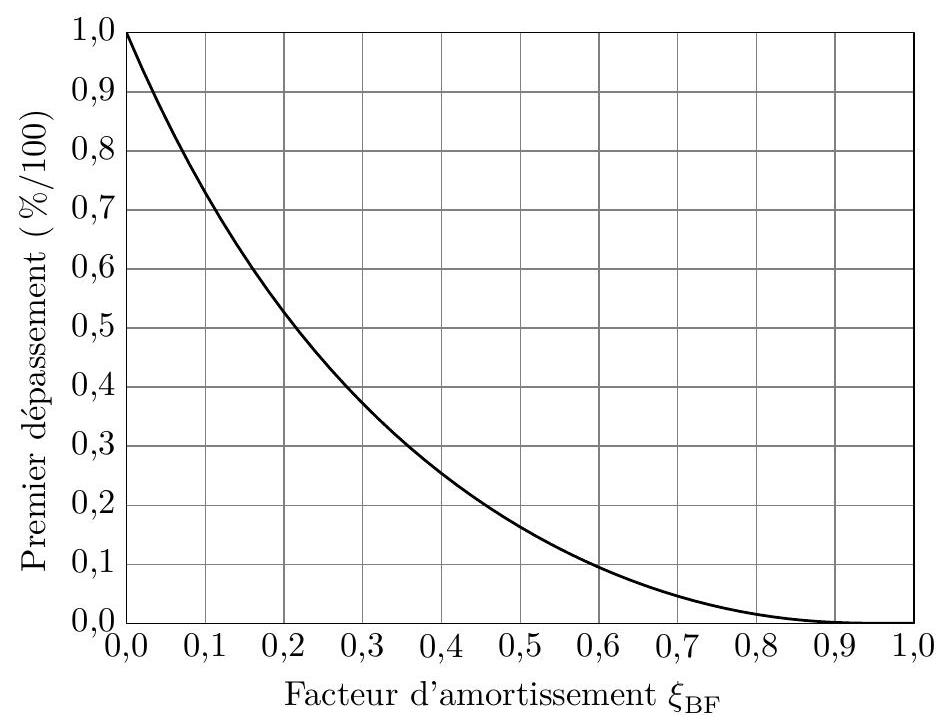
\includegraphics[width=.7\textwidth]{2025_07_06_ec63d2f3afc18cdeeb83g-07}
%Figure 9 
\caption{\label{ccs_mp_2022_fig_09}Abaque du premier dépassement}
\end{figure}
\fi


%III.B - 
\subsection{Introduction d'une correction \label{ccs_mp_2022_sec_3B}}

\begin{obj}
Pour pallier le non-respect de certaine(s) performance(s) du diagramme des exigences (figure \ref{ccs_mp_2022_fig_A}) sur le modèle $\mathrm{n}^{\circ} 1$ (figure \ref{ccs_mp_2022_fig_20}), le bureau d'études a choisi de mettre en place un correcteur dans la chaine directe, ou chaine d'action. L'objectif est de valider le choix du correcteur ainsi que son dimensionnement.
\end{obj}

%III.B.1) 
\subsubsection{Réglage d'un correcteur proportionnel vis-à-vis du critère de précision \label{ccs_mp_2022_sec_3B1}}

%Q 21. 
\question{\label{ccs_mp_2022_sec_q_21}À partir de l'expression de $\varepsilon_{a}$ déterminée à la question 19 montrer qu'un correcteur proportionnel de gain pur $K_{\text {corr.gain.pur }}$ placé dans la chaine directe, ou chaine d'action, permet d'améliorer l'erreur relative observée à la question 20.}
\ifprof
\begin{corrige}

On a $\varepsilon_\text{acc} =  \dfrac{0.3 g}{1+K_\text{BO}} $, donc si on ajoute un correcteur de type gain pur, l'erreur d'accélération deviendra :

$$\varepsilon_\text{acc} =  \dfrac{0.3 g}{1+ K_\text{corr. gain pur} \times K_\text{BO} } $$

 L'objectif étant de diminuer cette erreur, on voit que ce gain pur devra donc être supérieur à $1$. Ceci améliorera alors l'erreur relative observée à la question \ref{ccs_mp_2022_sec_q_20}.

\end{corrige}
\else
\fi


%Q 22. 
\question{\label{ccs_mp_2022_sec_q_22}Déterminer la valeur de $K_{\text {corr.gain.pur }}$ permettant d'atteindre l'exigence Id $=1.1 .1 .2 .1$.}
\ifprof
\begin{corrige}
On cherche à avoir $\varepsilon_\text{relatif} < 10\%$, d'où d'après la question \ref{ccs_mp_2022_sec_q_20} et \ref{ccs_mp_2022_sec_q_21} :
$ \varepsilon_\text{relatif} = \dfrac{1}{1 + K_\text{corr. gain pur} \times K_\text{BO}} < 0.1$
et $  1 + K_\text{corr. gain pur} \times K_\text{BO}  > \dfrac{1}{0.1} = 10$. Enfin 
$ K_\text{corr. gain pur} > \dfrac{9}{K_\text{BO}}$

A.N. : $ K_\text{corr. gain pur} > \dfrac{9}{8.4\times 10^{-3}} = 1071.4$.\end{corrige}
\else
\fi



%III.B.2) 
\subsubsection{Réglage d'un correcteur proportionnel vis-à-vis du critère de dépassement \label{ccs_mp_2022_sec_3B2}}
%Q 23. 
\question{\label{ccs_mp_2022_sec_q_23}À partir de l'expression de $\xi_{\mathrm{BF}}$ déterminée à la question \label{ccs_mp_2022_sec_q_17}, montrer qu'un correcteur proportionnel de gain pur $K_{\text {corr.gain.pur }}$ placé dans la chaine directe, ou chaine d'action, a une influence sur le dépassement observé à la question \label{ccs_mp_2022_sec_q_18}. Préciser alors le sens de variation du dépassement en fonction du gain $K_{\text {corr.gain.pur }}$.}
\ifprof
\begin{corrige}
On avait en question 18 : $\xi_\text{BF} = \dfrac{\xi_\text{BO}}{\sqrt{1 + K_\text{BO}}}$, en ajoutant un correcteur proportionnel de gain pur, le coefficient d'amortissement devient :
$ \xi_\text{BF} = \dfrac{\xi_\text{BO}}{\sqrt{1 + K_\text{corr. gain pur} \times K_\text{BO}}}$.

On remarque que plus le $K_\text{corr. gain pur}$ augmente (lorsqu'il est supérieur à $1$), plus le facteur d'amortissement diminue, ce qui implique que le dépassement sera plus important (d'après la \textsc{Figure} \ref{fig:sled9}).
\end{corrige}
\else
\fi


%Q 24. 
\question{\label{ccs_mp_2022_sec_q_24}Vérifier si l'exigence Id $=1.1 .1 .1 .2$ est respectée avec la valeur de $K_{\text {corr.gain.pur }}$ déterminée à la question \label{ccs_mp_2022_sec_q_22}.}
\ifprof
\begin{corrige}
$ \xi_\text{BF} = \dfrac{\xi_\text{BO}}{\sqrt{1 + K_\text{corr. gain pur} \times K_\text{BO}}} $
A.N. : $ \xi_\text{BF} = \dfrac{0.5}{\sqrt{1 + 476.2 \times 8.4 \times 10^{-3}}} \simeq  0.13 $.

\`A l'aide de la \textsc{Figure} \ref{fig:sled9}, on obtient un premier dépassement d'environ $0.62$, soit $62\%$.

L'exigence \texttt{Id = 1.1.1.1.2} (dépassement inférieur à $20\%$) n'est donc toujours pas respectée.

\end{corrige}
\else
\fi


%III.B.3) 
\subsubsection{Choix et réglage d'un correcteur proportionnel-intégral \label{ccs_mp_2022_sec_3B3}}
Le correcteur choisi par les ingénieurs du bureau d'études est un correcteur proportionnel-intégral, noté PI, de la forme

$$
C(p)=K_{\text {corr }}\left(\frac{1+T_{\text {corr }} p}{T_{\text {corr }} p}\right)=K_{\text {corr }}\left(1+\frac{1}{T_{\text {corr }} p}\right)=K_{\text {corr }}\left(1+\frac{\omega_{\text {corr }}}{p}\right) .
$$

%Q 25. 

\question{\label{ccs_mp_2022_sec_q_25}À l'aide des sections \ref{ccs_mp_2022_sec_3B1} et \ref{ccs_mp_2022_sec_3B2}, indiquer en quoi l'utilisation d'un correcteur proportionnel n'est pas suffisante dans le cas du Sled. Justifier le choix d'un correcteur proportionnel-intégral.}
\ifprof
\begin{corrige}
On a vu en section 3.2.1 qu'avec un correcteur proportionnel permettait de respecter l'exigence \texttt{Id = 1.1.1.2.1} concernant l'écart relatif. Mais en section 3.2.2 on s'est aperçu que le critère de dépassement (exigence \texttt{Id = 1.1.1.1.2}) ne peut être respecté (car il faudrait diminuer $K_\text{corr. gain pur}$ pour diminuer le dépassement, mais cela impliquerait que nous perdions le respect de l'exigence de précision sur l'écart relatif).\\

Un correcteur proportionnel-intégral permet d'augmenter la classe de la FTBO et donc d'avoir $\varepsilon_\text{relatif} = 0$ et cela indépendamment de la valeur de $K_\text{corr. gain pur}$. Ainsi on peut régler $K_\text{corr. gain pur}$ afin de respecter l'exigence de dépassement \texttt{Id = 1.1.1.1.2}.
\end{corrige}
\else
\fi



%Q 26. 
\question{\label{ccs_mp_2022_sec_q_26}Tracer sur la copie le diagramme asymptotique de la phase du diagramme de Bode théorique du correcteur proportionnel-intégral. Préciser ses caractéristiques principales. Compléter le diagramme asymptotique de la phase avec l'allure du diagramme réel de phase du correcteur.}
\ifprof
\begin{corrige}
La phase du correcteur s'écrit :
$\begin{array}{ll}
\varphi &= \text{arg}(K_\text{corr}) + \text{arg}\left(\dfrac{1 + j T_\text{corr} \omega}{j T_\text{corr} \omega}\right)\\
	&= 0 + \text{arctan}\left( T_\text{corr} \omega\right) - \text{arg}\left(j T_\text{corr} \omega\right)\\
	&= -90 +\text{arctan}\left( T_\text{corr} \omega\right)
\end{array}$

On obtient alors le diagramme de Bode suivant pour la phase :
%\begin{figure}[h!]
%\begin{tikzpicture}
%\begin{semilogxaxis}[domain=10^-1:10^5,  samples=200,  grid=both,  no markers, enlarge x limits=false, enlarge y limits=false,
%            ylabel = Phase [$\degres$\text{]},
%            xlabel = $\omega$ [rad/s\text{]},
%             width=.95\textwidth,
%             height=.5\textwidth,
%             ymin=-97, ymax=10.5,
%             ytick={0,-22,-45,-67,-90}]
%\foreach \K in {3} \foreach \tau in {0.02} {
%	\plot[blue,smooth,ultra thick, declare function={phase(\p,\a,\b)=-90+atan(\b*\p);}] 
%	(\x, {phase(\x,\K,\tau)});
%	\addplot [green, ultra thick, dashed] coordinates {(10^-1, -90) (1/\tau, -90) (1/\tau, 0) (10^5, 0)};
%	\addplot [green, thick, opacity=0] coordinates {(1/\tau, -90) (1/\tau,-45)} node[midway, anchor=north, inner sep=5, sloped, opacity=1] {\color{black}$\omega_\text{cassure} = 1/T_\text{corr}$} ;
%	\addplot [black, ultra thick, ->, >=latex] coordinates {(10/\tau, -5.7) (10/\tau,0)} node[midway, anchor=south, inner sep=5, sloped] {\color{black}$5.7\degres$} ;
%}
%\end{semilogxaxis}
%\end{tikzpicture}
%\end{figure}

\end{corrige}
\else
\fi

\ifprof
\else
Dans un premier temps, le bureau d'études souhaite régler le correcteur proportionnel-intégral afin que le modèle $\mathrm{n}^{\circ} 1$ corrigé puisse atteindre les performances de stabilité définies dans le diagramme des exigences (figure \ref{ccs_mp_2022_fig_A}). Pour cela, il utilise un programme codé en Python (figure \ref{ccs_mp_2022_fig_10}).
\begin{figure}
\centering
\begin{lstlisting}
import numpy as np

def H_BO_nc(Omega):
    # Définition de la fonction de transfert en boucle ouverte non corrigée
    K_BO = 8.4e-3 # gain en boucle ouverte non corrigée
    omegaO_BO = 71 # pulsation propre en boucle ouverte non corrigée
    Xi_BO = 0.5 # facteur d'amortissement en boucle ouverte non corrigée
    u = Omega/omegaO_BO # pulsation réduite
    FTBO_nc = K_BO/(1 + 2*Xi_BO*(1j*u) - u**2)
    return FTBO_nc
    
def reglage_PI(H_BO_nc,M_phi):
    # Détermination des paramètres du correcteur P.I. à l'aide de deux paramètres :
    # H_BO_nc : Fonction de transfert en BO du système non corrigé
    # M_phi : Marge de phase souhaitée après réglage du correcteur
    epsilon=0.5
    pas = 0.001
    Omega= 10**np.arange(0,3+pas,pas) # Pulsation de 10^0 à 10^3 en rad.s-1
    GdB_BO_nc = 20*np.log10(np.absolute(H_BO_nc(Omega))) # Gain en dB de la fonction
            # en BO non corrigée
    Phi_BO_nc = np.angle(H_BO_nc(Omega),'deg') # Phase en * de la fonction
            # en BO non corrigée
    Phi_recherchée_avant_correction= M_phi - 180 + 5.7
    i=0
    while i<len(Phi_BO_nc) and abs(Phi_BO_nc[i]-Phi_recherchée_avant_correction)>epsilon:
        i=i+1
    if i!=len(Phi_BO_nc):
        Omega_corr=Omega[i]/10 # Calcul de la pulsation de cassure du correcteur
        T_corr=1/Omega_corr # Calcul de la constante de temps du correcteur
        K_corr=10**(-GdB_BO_nc[i]/20)# Calcul du gain du correcteur
        return K_corr,T_corr
\end{lstlisting}

%Figure 10 
\caption{\label{ccs_mp_2022_fig_10}Code python de détermination du réglage du correcteur PI}
\end{figure}

\section*{Notations}
\begin{itemize}
  \item $\Phi\left(H_{\mathrm{BOnc}}\left(\omega_{c 0 \mathrm{~dB}}\right)\right)$ la phase de la boucle ouverte non corrigée à la pulsation de coupure à 0 dB .
  \item $\Phi\left(H_{\mathrm{BO}}\left(\omega_{c 0 \mathrm{~dB}}\right)\right)$ la phase souhaitée de la boucle ouverte corrigée à la pulsation de coupure à 0 dB .
  \item $M P$ la marge de phase souhaitée après correction.
\end{itemize}
\fi


%Q 27. 
\question{\label{ccs_mp_2022_sec_q_27}
Exprimer $\Phi\left(H_{\mathrm{BO}}\left(\omega_{c} 0 \mathrm{~dB}\right)\right)$ en fonction de $M P$.}
\ifprof
\begin{corrige}
$\Phi(H_\text{BO}(\omega_{c \text{0 dB}})) = -180\degres + M P$
\end{corrige}
\else
\fi

%Q 28. 
\question{\label{ccs_mp_2022_sec_q_28}Exprimer $\Phi\left(H_{\mathrm{BO}}\left(\omega_{c} 0 \mathrm{~dB}\right)\right)$ en fonction de $\Phi\left(H_{\mathrm{BO} \mathrm{nc}}\left(\omega_{c} 0 \mathrm{~dB}\right)\right)$, de $T_{\text {corr }}$ et de $\omega_{c} 0 \mathrm{~dB}$.}
\ifprof
\begin{corrige}
$\Phi(H_\text{BO}(\omega_{c \text{0 dB}})) = \Phi(H_\text{BO nc}(\omega_{c \text{0 dB}})) - 90\degres + \text{arctan}(T_\text{corr} \omega_{c \text{0 dB}})$
\end{corrige}
\else
\fi

%Q 29. 
\question{\label{ccs_mp_2022_sec_q_29}En déduire l'expression de $\Phi\left(H_{\mathrm{BO} \mathrm{nc}}\left(\omega_{c 0 \mathrm{~dB}}\right)\right)$ en fonction de $M P$, de $T_{\text {corr }}$ et de $\omega_{c 0 \mathrm{~dB}}$.}
\ifprof
\begin{corrige}
$\Phi(H_\text{BO nc}(\omega_{c \text{0 dB}})) = -90\degres + M P - \text{arctan}(T_\text{corr} \omega_{c \text{0 dB}})$.
\end{corrige}
\else
\fi

%Q 30. 
\question{\label{ccs_mp_2022_sec_q_30}Préciser comment est déterminée la pulsation de cassure du correcteur dans la méthode décrite dans le code Python de la figure \ref{ccs_mp_2022_fig_10} (ligne 26).}
\ifprof
\begin{corrige}
La pulsation de cassure du correcteur est choisi à une décade de la pulsation de coupure à $0$ dB de la fonction de transfert non corrigée. Cela implique un déphasage au niveau de la pulsation de coupure à $0$ dB de $5.7\degres$, ce qui a été pris en compte ligne 21.
\end{corrige}
\else
\fi


%Q 31. 
\question{\label{ccs_mp_2022_sec_q_31}À l'aide de l'étude précédente menée sur la correction retrouver la valeur $5,7^{\circ}$ utilisée ligne 21 dans la méthode décrite dans le code Python de la figure \ref{ccs_mp_2022_fig_10}.}
\ifprof
\begin{corrige}
En se plaçant à une décade de la pulsation de cassure du correcteur (qui est la phase de coupure à $0$ dB de la fonction de transfert non corrigée), on obtient une phase de :
$ \phi = -90 + \text{arctan}\left({T_\text{corr}} \times \dfrac{10}{{T_\text{corr}}}\right) = -90 + \text{arctan}(10) = -90 + 84.29 = -5.69\degres$.
\end{corrige}
\else
\fi

%Q 32. 
\question{\label{ccs_mp_2022_sec_q_32}Représenter cette valeur sur le tracé du diagramme de Bode de la phase du correcteur PI (question 26) et indiquer à quoi correspond cette valeur.}
\ifprof
\begin{corrige}
Cette valeur correspond au déphasage induit par l'ajout d'un correcteur dont la pulsation de cassure est située à une décade avant la pulsation de coupure à $0$ dB de la fonction de transfert non corrigée. Pour régler la marge de phase d'une fonction de transfert avec un correcteur PI par la méthode du décalage à une décade, il faut prendre en compte et régler une marge de phase de :
$M P = M P_\text{voulue} + 5.7\degres$.

Ce qui permet d'anticiper le déphasage du correcteur PI.
\end{corrige}
\else
\fi

\ifprof
\else
En utilisant la méthode de réglage du correcteur décrite dans le code Python (figure \ref{ccs_mp_2022_fig_10}), les paramètres du correcteur ont été déterminés. Les ingénieurs ont retenu les valeurs $K_{\text {corr }}=354$ et $T_{\text {corr }}=1 / 15 \mathrm{~s}=0,066 \mathrm{~s}$. La figure \ref{ccs_mp_2022_fig_11} représente le diagramme de Bode de la boucle ouverte de l'asservissement en vitesse du modèle $n^{\circ} 1$ ainsi corrigé.
\fi

%III.B.4) 
\subsubsection{Validation des exigences \label{ccs_mp_2022_sec_3B4}}
La réponse temporelle en accélération, du modèle $n^{\circ} 1$ corrigé, en réponse à la consigne d'accélération définie figure \ref{ccs_mp_2022_fig_04} est donnée sur la figure \ref{ccs_mp_2022_fig_12}.

%Q 33. 
\question{\label{ccs_mp_2022_sec_q_33}Évaluer graphiquement la marge de phase du système corrigé et conclure au regard de l'exigence Id = 1.1.1.1.1.}
\ifprof
\begin{corrige}
On lit graphiquement une marge de phase d'environ :$ M P = 42\degres > 30\degres \qquad \text{exigence \texttt{Id : 1.1.1.1.1}}$.

Ce qui respecte l'exigence \texttt{Id : 1.1.1.1.1}.
\end{corrige}
\else
\fi

%Q 34. 
\question{\label{ccs_mp_2022_sec_q_34}Évaluer le premier dépassement suite à l'échelon de consigne de $0,3 g$ et conclure au regard de l'exigence $\mathrm{Id}=1.1 .1 .1 .2$.}
\ifprof
\begin{corrige}
Le premier dépassement que l'on peut observer en \textsc{Figure} \ref{fig:sled12} est de :

$$ D_\% = \dfrac{3.6 - 3}{3} \times 100 = 0.2 \times 100 = 20\%$$

En ayant pris $3.6$ m.s$^{-2}$, nous avons surestimé la mesure, on peut donc valider l'exigence \texttt{Id : 1.1.1.1.2} qui impose un dépassement inférieur à $20\%$.
\end{corrige}
\else
\fi

%Q 35. 
\question{\label{ccs_mp_2022_sec_q_35}Conclure, en justifiant, au regard de l'exigence $\mathrm{Id}=1.1 .1 .2 .1$.}
\ifprof
\begin{corrige}
La précision indicielle est de :
$ \text{précision} = \dfrac{|0.3\times g - 3.0|}{0.3 \times g} = \left|1 - \dfrac{3.0}{0.3 \times g} \right| = \left|1 - \dfrac{10}{g}\right|$.

A.N. : $ \text{précision} = \left|1 -\dfrac{10}{9.81}\right| = 0.019 = 1.9\% < 10\% \qquad \text{exigence \texttt{Id : 1.1.1.2.1}}$.

On ne peut pas valider toutes les exigences avec les études réalisées jusqu'ici, mais les exigences \texttt{Id : 1.1.1.1.1}, \texttt{Id : 1.1.1.1.2} et \texttt{Id : 1.1.1.2.1} sont validées avec un correcteur PI réglé à une décade.
\end{corrige}
\else
\fi


\ifprof
\else
\begin{figure}[!h]
\centering
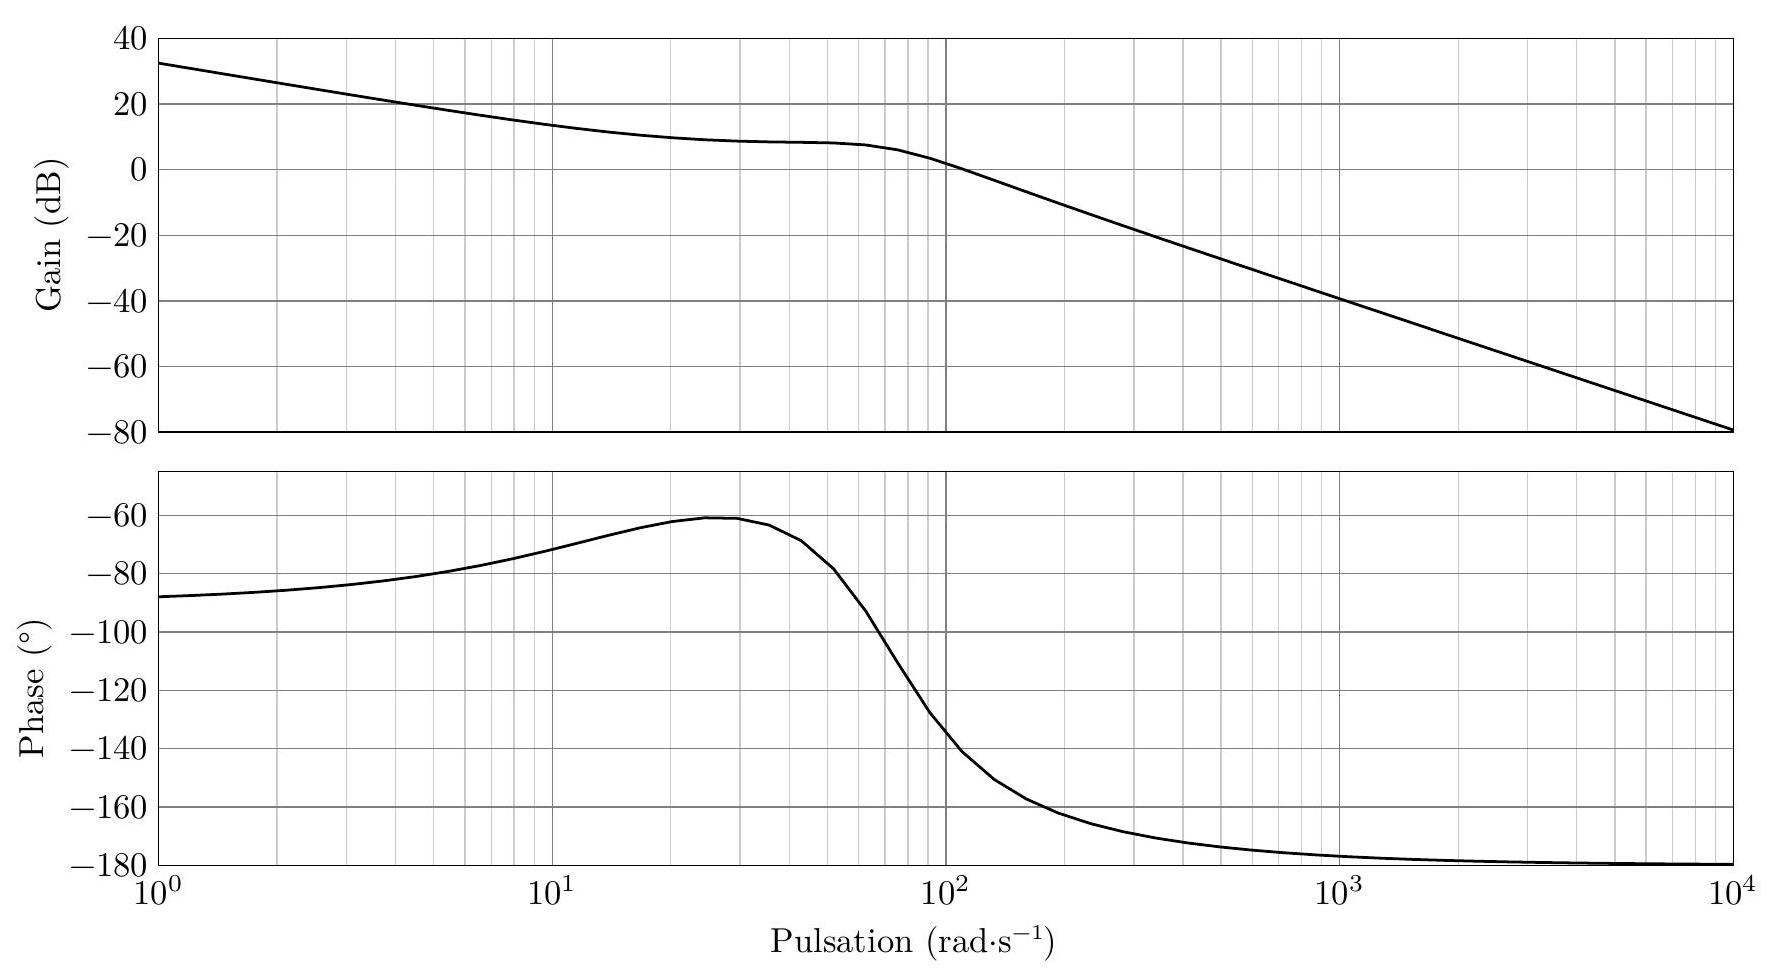
\includegraphics[width=\textwidth]{2025_07_06_ec63d2f3afc18cdeeb83g-09}

%Figure 11 
\caption{\label{ccs_mp_2022_fig_11}Diagramme de Bode de la boucle ouverte de l'asservissement en vitesse avec correction}
\end{figure}

\begin{figure}[!h]
\centering
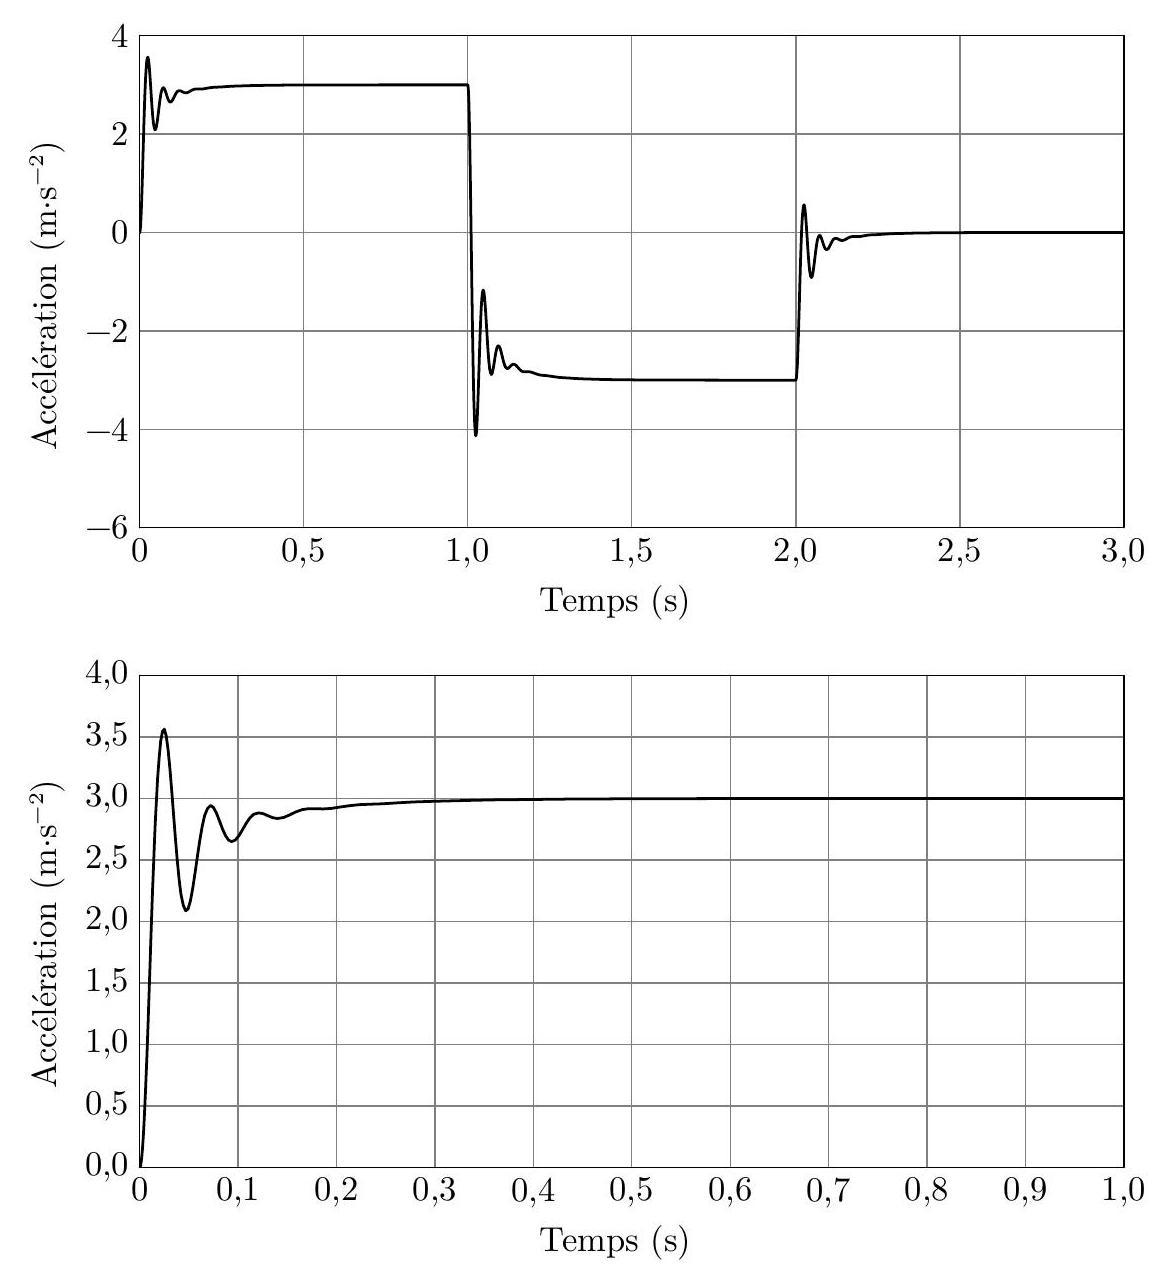
\includegraphics[width=\textwidth]{2025_07_06_ec63d2f3afc18cdeeb83g-09(1)}

%Figure 12 
\caption{\label{ccs_mp_2022_fig_12}Réponse temporelle en accélération du système corrigé (au-dessus) et zoom (en dessous) sur l'échelon de consigne $0,3 g$}
\end{figure}

Les ingénieurs du bureau d'études décident d'arrêter en l'état la modélisation du Sled $0,3 g$ qui a permis de définir une première structure de commande. Ils souhaitent à présent s'investir dans la réalisation d'un Sled et mener des expérimentations.
\fi

%IV 
\section{Réalisation d'un Sled $\mathbf{0 , 3 g}$ \label{ccs_mp_2022_sec_4}}

\ifprof
\else
En tenant compte des résultats du prédimensionnement et de la modélisation, un prototype du Sled $0,3 g$ a été réalisé par le bureau d'études et mis en place dans le laboratoire d'expérimentations (figure \ref{ccs_mp_2022_fig_13}). Les résultats obtenus avec ce prototype devront vérifier les exigences définies dans le diagramme (figure \ref{ccs_mp_2022_fig_A}). Ils pourront également être confrontés aux résultats issus de la modélisation. Cela permettra, à terme, de faire évoluer à la fois le modèle numérique et le prototype.\\


\begin{figure}[!h]
\centering
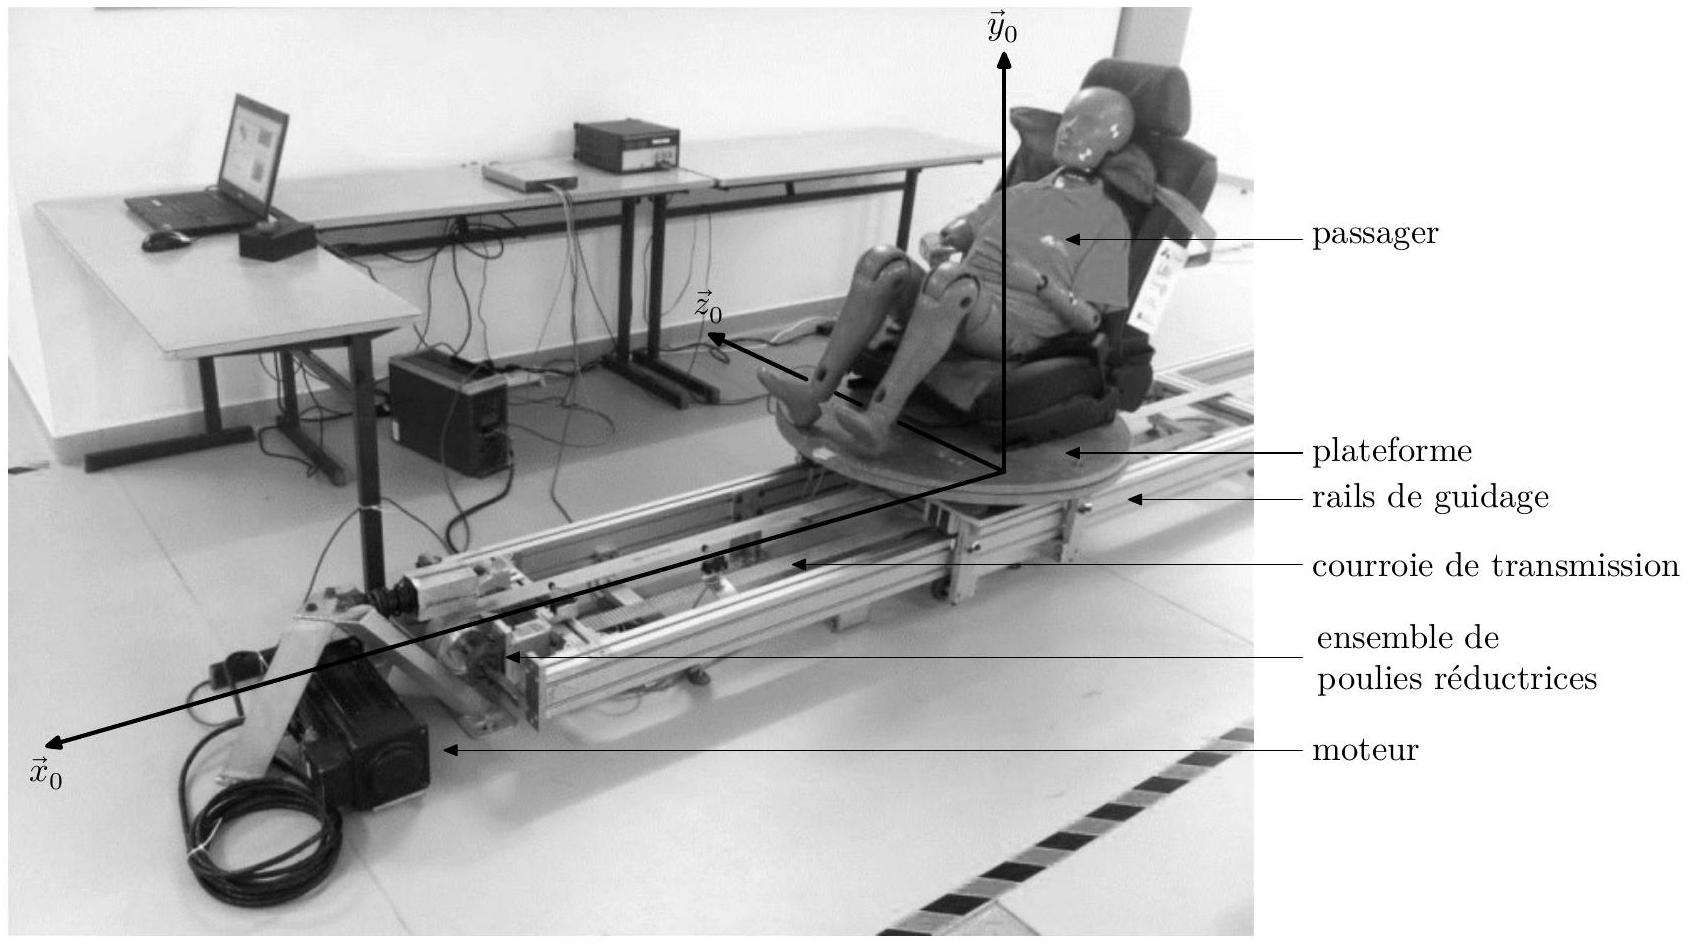
\includegraphics[width=.7\textwidth]{2025_07_06_ec63d2f3afc18cdeeb83g-10(1)}

%Figure 13 
\caption{\label{ccs_mp_2022_fig_13}Prototype du Sled (ou dispositif expérimental) à $0,3 g$}
\end{figure}
\fi

%IV.A - 
\subsection{Validation du choix de la motorisation effectué par le bureau d'études \label{ccs_mp_2022_sec_4A}}

\ifprof
\else
\begin{obj}
Dans un premier temps, il s'agit de valider le choix du moteur électrique retenu par les ingénieurs pour motoriser le prototype du Sled et répondre aux exigences.
\end{obj}

\subsubsection*{Hypothèses d'étude}
Compte tenu des dimensions du Sled définies lors du prédimensionnement, la chaine de transmission de puissance du moteur à l'ensemble mobile $S$ a été conçue et réalisée avec un système de poulies et de courroies comme représenté sur la figure \ref{ccs_mp_2022_fig_14}.

\begin{figure}[!h]
\centering
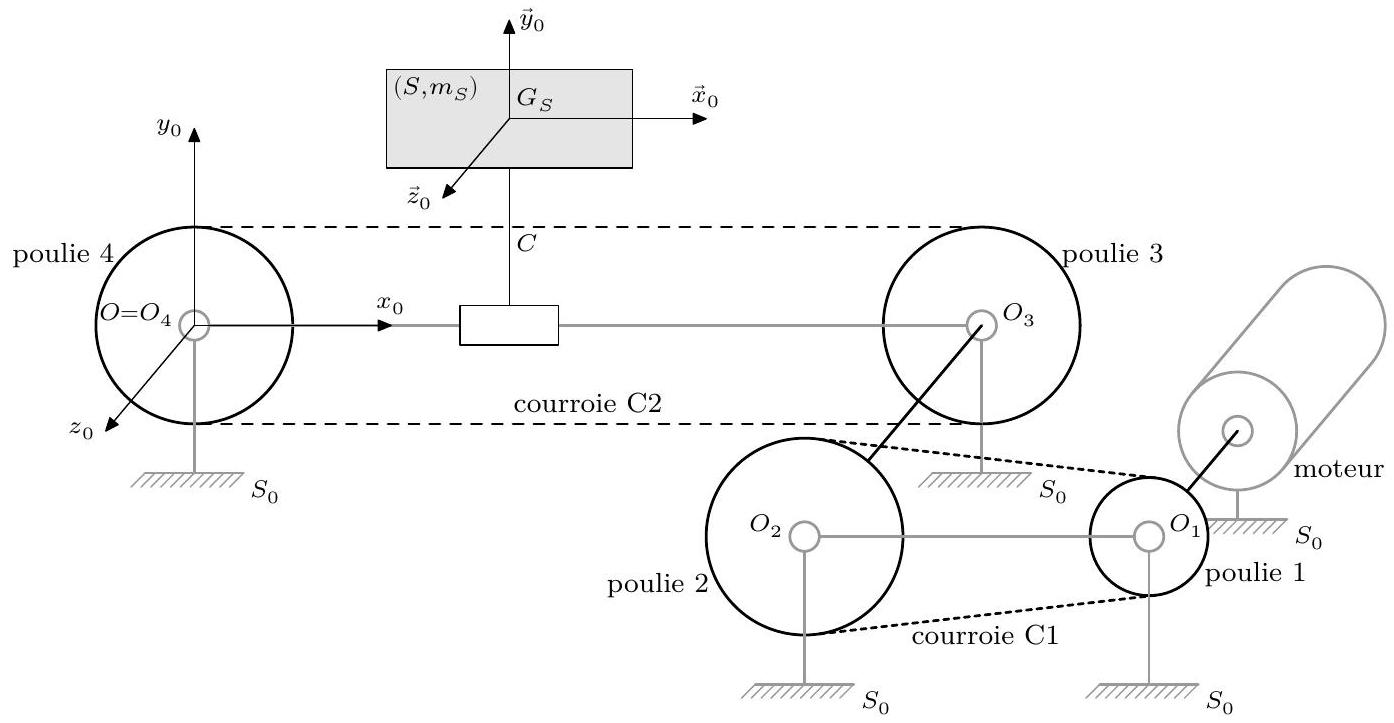
\includegraphics[width=.7\textwidth]{2025_07_06_ec63d2f3afc18cdeeb83g-10}

%Figure 14 
\caption{\label{ccs_mp_2022_fig_14}Modélisation cinématique de la chaine de transmission de puissance du prototype du Sled}
\end{figure}

Les poulies 1, 2 et la courroie C1 réalisent une adaptation de la vitesse de rotation en sortie du moteur électrique. Les poulies 3, 4 et la courroie C2 participent à la transformation de mouvement de rotation des poulies en mouvement de translation de l'ensemble mobile $S$.\\
Sur le prototype du Sled, le rendement global de la chaine de transmission de puissance prenant en compte tous les frottements (sec et fluide) est estimé à $\eta=55 \%$. La puissance totale ainsi perdue, notée $P_{\text {frottement }}$, s'exprime en fonction de la puissance fournie par le moteur : $P_{\text {frottement }}=(1-\eta) P_{\text {stator } \rightarrow \text { rotor } / S_{0}}$.

\subsubsection*{Notations et données}
\begin{itemize}
  \item $m_{S}$, masse de l'ensemble mobile $S=\{$ volontaire + siège + plateforme + capteurs $\}$.
  \item $t$, le temps, exprimé en secondes.
  \item $\vec{V}_{\left(G_{S}, S / S_{0}\right)}=v(t) \vec{x}_{0}$, la vitesse de déplacement du centre de gravité $G_{S}$ de l'ensemble mobile $S$ par rapport au bâti $S_{0}$.
  \item $J_{P_{1}}$, le moment d'inertie du sous-ensemble $P_{1}=\{$ poulie $1+$ rotor moteur $\}$ autour de son axe de rotation $\left(O_{1}, \vec{z}_{0}\right)$.
  \item $\vec{\Omega}_{\left(P_{1} / S_{0}\right)}=\omega_{1}(t) \vec{z}_{0}$, la vitesse angulaire de rotation d'axe ( $O_{1}, \vec{z}_{0}$ ) du sous-ensemble $P_{1}$ par rapport au bâti $S_{0}$.
  \item $\vec{C}_{m}=C_{m}(t) \vec{z}_{0}$, le couple exercé par le stator, lié à $S_{0}$, sur le rotor du moteur d'axe ( $O_{1}, \vec{z}_{0}$ ), avec $C_{m \text { max }}=$ $32 \mathrm{~N} \cdot \mathrm{~m}$ (donnée constructeur).
  \item $J_{P_{2}}$, le moment d'inertie équivalent du sous-ensemble $P_{2}=\{$ poulie $2+$ arbre de transmission + poulie $3+$ poulie $4+$ courroie C 2$\}$, rapporté à l'axe de rotation $\left(O_{2}, \vec{z}_{0}\right)$.
  \item $\vec{\Omega}_{\left(P_{2} / S_{0}\right)}=\omega_{2}(t) \vec{z}_{0}$, la vitesse angulaire de rotation de ce sous-ensemble $P_{2}$ par rapport au bâti $S_{0}$ autour de l'axe de rotation ( $O_{2}, \vec{z}_{0}$ ).
  \item $D_{2}=D_{3}=D_{4}=100 \mathrm{~mm}$, les diamètres des poulies 2,3 et 4 .
  \item $D_{1}=35 \mathrm{~mm}$, le diamètre de la poulie 1 .
  \item La masse et le moment d'inertie de la courroie C 1 sont négligés.
\end{itemize}
\fi

%Q 36. 
\question{\label{ccs_mp_2022_sec_q_36}Déterminer le rapport $k=\frac{\omega_{1}(t)}{\omega_{2}(t)}$.}
\ifprof
\begin{corrige}
$ k = \dfrac{\omega_1(t)}{\omega_2(t)} = \dfrac{D_2}{D_1}$ (en considérant une vitesse de glissement nulle entre la courroie et les poulies $1$ et $2$).
A.N. $ k = \dfrac{100}{35} \simeq 2.86$

C'est le rapport de transmission entre la poulie $1$ (en entrée) et la poulie $2$ (en sortie).
\end{corrige}
\else
\fi

%Q 37. 
\question{\label{ccs_mp_2022_sec_q_37}Déterminer $v(t)$ en fonction de $\omega_{1}(t)$ et d'un paramètre géométrique. Préciser les hypothèses nécessaires à la détermination de $k$ et de la relation entre $v(t)$ et $\omega_{1}(t)$.}
\ifprof
\begin{corrige}
$v(t) = \overrightarrow{V}_{G_S, S/S_0} \cdot \vec x_0$, or $\overrightarrow{V}_{G_S, S/S_0} = \overrightarrow{V}_{C, S/S_0} = \overrightarrow{V}_{C, C2/S_0} = \overrightarrow{V}_{I, C2/S_0} = \overrightarrow{V}_{I, \text{poulie } 3/S_0}$ (en considérant une vitesse de glissement nulle entre la poulie $3$ et la courroie C2).\\

Avec $I$ le point de contact entre la courroie C2 et la poulie $3$.

$\overrightarrow{V}_{I, \text{poulie } 3 /S_0} = \overrightarrow{V}_{O_3, \text{poulie } 3/S_0} + \overrightarrow{IO_3} \wedge \overrightarrow{\Omega}_{(P_3/S_0)}$

Or $\overrightarrow{\Omega}_{(P_3/S_0)} = \overrightarrow{\Omega}_{(P_2/S_0)} = \omega_2(t) \vec z_0$ \qquad car $\overrightarrow{\Omega}_{(P_3/P_2)} = \overrightarrow 0$

$\overrightarrow{V}_{I, \text{poulie } 3 /S_0} = \overrightarrow 0 + (-\dfrac{D_3}{2} \vec y_0) \wedge \omega_2(t) \vec z_0 = -\dfrac{D_3}{2} \omega_2(t) \vec x_0$, soit d'après la question 36 :
$ v(t) = - \dfrac{D_3 \, \omega_1(t)}{2 \, k}$.
\end{corrige}
\else
\fi


%Q 38. 
\question{\label{ccs_mp_2022_sec_q_38}En fonction de $\omega_{1}(t)$, exprimer l'énergie cinétique dans leur mouvement par rapport à $R_{0}\left(O, \vec{x}_{0}, \vec{y}_{0}, \vec{z}_{0}\right)$, repère supposé galiléen attaché à $S_{0}$, de}


\begin{itemize}
  \item la classe d'équivalence du sous-ensemble noté $P_{1}: E_{c}\left(P_{1} / S_{0}\right)$;
  \item la classe d'équivalence du sous-ensemble noté $P_{2}: E_{c}\left(P_{2} / S_{0}\right)$;
  \item la classe d'équivalence de l'ensemble mobile $S: E_{c}\left(S / S_{0}\right)$.
\end{itemize}

\ifprof
\begin{corrige}
\begin{itemize}
\item $E_c(P_1/S_0) = \dfrac{1}{2} J_{P_1} \omega_1(t)^2$ ;
\item $E_c(P_2/S_0) = \dfrac{1}{2} J_{P_2} \omega_2(t)^2 = \dfrac{1}{2} J_{P_2} \dfrac{\omega_1(t)^2}{k^2} $ ;
\item $E_c(S/S_0) = \dfrac{1}{2} m_S v(t)^2 = \dfrac{1}{2} m_S  \dfrac{D_3^2 \, \omega_1(t)^2}{4 \, k^2}$.
\end{itemize}
\end{corrige}
\else
\fi

%Q39
\question{\label{ccs_mp_2022_sec_q_39}Exprimer le moment d'inertie équivalent rapporté à l'axe moteur ( $O_{1}, \vec{z}_{0}$ ), noté $J_{\text {eq }}$, de la chaine de transmission de puissance composée des sous-ensembles $P_{1}, P_{2}$ et de l'ensemble mobile $S$, en fonction de $k, D_{1}$ et des différentes données inertielles propres à chaque classe d'équivalence.}
\ifprof
\begin{corrige}
$\begin{array}{ll}
E_c(\{P_1+P_2+S\}/S_0) &= \dfrac{1}{2} \left(  J_{P_1} + \dfrac{J_{P_2}}{k^2} + \dfrac{m_S D_3^2}{4 k^2}\right) \omega_1(t)^2 \\
&= \dfrac{1}{2} J_\text{eq} \omega_1(t)^2 \\
\end{array}$

Le rapport de transmission nous permet également d'écrire : $D_3 = D_2 = k \times D_1$

Finalement, on a : $ J_\text{eq} = J_{P_1} + \dfrac{J_{P_2}}{k^2} + m_S D_1^2$.
\end{corrige}
\else
\fi
%Q40
\question{\label{ccs_mp_2022_sec_q_40}Déterminer le couple $C_{m}(t)$. Il est attendu de préciser le système isolé, de détailler l'inventaire des différentes puissances intérieures et extérieures mises en jeu en les distinguant clairement, d'indiquer également les puissances qui sont nulles, en donnant une justification, et de donner l'expression du théorème utilisé.}
\ifprof
\begin{corrige}
On isole le système : \{ $P_1 + P_2 + S$ \}

Le bilan des puissances internes et externes est :
\begin{itemize}
\item $P_\text{externe} = P_\text{stator $\to$ rotor $/S_0$} = P_m = C_m \times \omega_1(t)$ ;
\item $P_\text{interne} = -P_\text{frottement} = -(1 - \eta) P_m$.\\
\end{itemize}

D'après le théorème de l'énergie cinétique (ou théorème de l'énergie puissance) appliqué au système isolé (et à l'aide de la question 39), on obtient la relation finale :

$ \dfrac{\text{d} E_c(P_1+P_2+S/S_0)}{\text{d}t} = P_\text{externe} + P_\text{interne}$
$ \Rightarrow  J_\text{eq} \dot\omega_1(t) \omega_1(t) = P_m  - (1 - \eta) P_m$
$ \Rightarrow  J_\text{eq} \dot\omega_1(t) {\omega_1(t)} = \eta C_m(t) \times {\omega_1(t)}$
$ \Rightarrow   C_m(t) = \dfrac{J_\text{eq}}{\eta} \dfrac{\text{d}\omega_1(t)}{\text{d}t}$.

\end{corrige}
\else
\fi

%Q 41. 
\question{\label{ccs_mp_2022_sec_q_41}Mettre $C_{m}(t)$ sous la forme $C_{m}(t)=\alpha \frac{\mathrm{d} v(t)}{\mathrm{d} t}$ en précisant l'expression de $\alpha$ en fonction de $J_{\text {eq }}, D_{1}$ et de $\eta$.\\
La suite du questionnement sera effectuée avec la valeur numérique $J_{\text {eq }}=0,064 \mathrm{~kg} \cdot \mathrm{~m}^{2}$.}
\ifprof
\begin{corrige}
D'après la question 37, on a : $\omega_1(t) = -\dfrac{2 \, k \, v(t)}{D_3} = -\dfrac{2 \, {k} \, v(t)}{{k} \, D_1} = -\dfrac{2 \, v(t)}{D_1} $, d'où :$ C_m(t) = - \dfrac{2 \, J_\text{eq}}{\eta \, D_1} \dfrac{\text{d}v(t)}{\text{d}t}$.
\end{corrige}
\else
\fi

%Q 42. 
\question{\label{ccs_mp_2022_sec_q_42}Tracer sur la copie, l'évolution du couple moteur en fonction du temps, correspondant au graphe de vitesse donné en figure \ref{ccs_mp_2022_fig_15}. Préciser les valeurs caractéristiques.}
\ifprof
\begin{corrige}
%\begin{center}
%	\begin{tikzpicture}
%	\coordinate (O) at (0,0);
%	\def \myxf{10}
%	\def \myyf{3.2}
%	\def \myU{2}
%	\def \mytz{5}
%		\draw [->,>=latex] ($(O)+(-.5,0)$) -- node[pos=1,anchor=west] {$t$ [s]} ($(O)+(\myxf+1,0)$) ;
%		\draw [->,>=latex] ($(O)+(0,-3.2)$) -- node[pos=1,anchor=south, blue] {$C_m(t)$}  ($(O)+(0,\myyf)$) ;
%		\draw[blue, thick] ($(O)+(0,-2)$) -- (\mytz,-2) -- (\mytz,\myU) -- (\myxf-.5,\myU); 
%		\draw[black] (0,-.1) -- node[pos=0,anchor=north east] {$0$} (0,.1);
%		\draw[black] (\mytz,-.1) -- node[pos=0,anchor=north east] {$1$} (\mytz,.1);
%		\draw[black] (\myxf,-.1) -- node[pos=0,anchor=north east] {$2$} (\myxf,.1);
%		\draw[black] (-.1,\myU) -- node[pos=0,anchor=east] {$\dfrac{2 \, J_\text{eq} \times 0.3 g}{\eta D_1}$} (.1,\myU);
%		\draw[black] (-.1,-\myU) -- node[pos=0,anchor=east] {$-\dfrac{2 \, J_\text{eq} \times 0.3 g}{\eta D_1}$} (.1,-\myU);
%
%	\end{tikzpicture}
%\end{center}

\end{corrige}
\else
\fi


\ifprof
\else


\begin{figure}[!h]
\centering
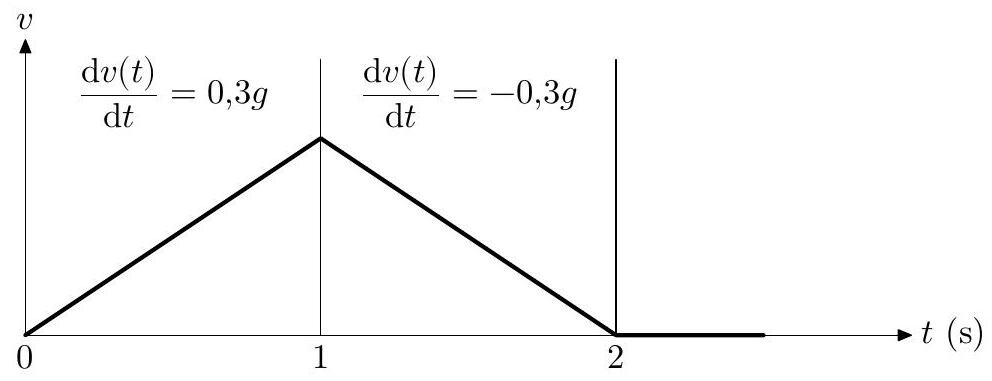
\includegraphics[width=.7\textwidth]{2025_07_06_ec63d2f3afc18cdeeb83g-11}

%Figure 15 
\caption{\label{ccs_mp_2022_fig_15}Évolution de la vitesse de l'ensemble mobile}
\end{figure}
\fi

%Q 43. 
\question{\label{ccs_mp_2022_sec_q_43}Conclure quant au choix de moteur effectué par les ingénieurs du bureau d'études sur ce critère de couple moteur.}
\ifprof
\begin{corrige}
Le moteur choisi par les ingénieurs permet de délivrer un couple maximal de : $C_{m\text{max}} = 32$ N.m.

Le couple moteur a un couple maximal d'après la \textsc{Figure} \ref{fig:sled15} de $C_m = \dfrac{2 \, J_\text{eq} \times 0.3 g}{\eta D_1}$.

A.N. :$ C_m = \dfrac{2 \times 0.064 \times 0.3 \times 9.81}{0.55 \times 35 \times 10^{-3}} \simeq 19.6 \text{ N.m}$.

Le moteur a donc été dimensionné avec un coefficient de sécurité de $1.5$. Le moteur choisi par les ingénieur peut fournir le couple nécessaire à l'évolution de la vitesse de l'ensemble mobile.
\end{corrige}
\else
\fi


%IV.B - 
\subsection{Analyse des essais réalisés sur le prototype du Sled pour les conditions $\pm 0,3 g$}

\begin{obj}
L'objectif est de vérifier si les performances du prototype ainsi motorisé sont conformes aux exigences (figure \ref{ccs_mp_2022_fig_A}).
\end{obj}
\ifprof
\else


Trois tests expérimentaux, avec une masse embarquée de 80 kg représentative d'un volontaire, ont été réalisés sur le prototype du Sled (figure \ref{ccs_mp_2022_fig_16}). La figure \ref{ccs_mp_2022_fig_17} représente les écarts relatifs entre les essais respectifs.\\


\begin{figure}[!h]
\centering
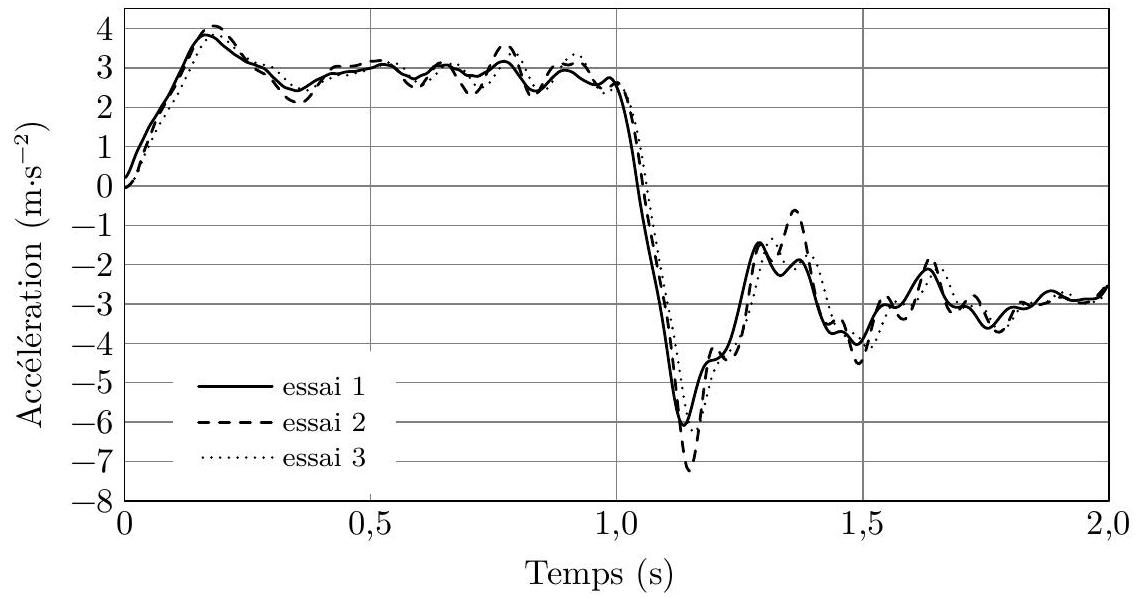
\includegraphics[width=\textwidth]{2025_07_06_ec63d2f3afc18cdeeb83g-12}
%Figure 16 
\caption{\label{ccs_mp_2022_fig_16}Résultats temporels des 3 essais}
\end{figure}


\begin{figure}[!h]
\centering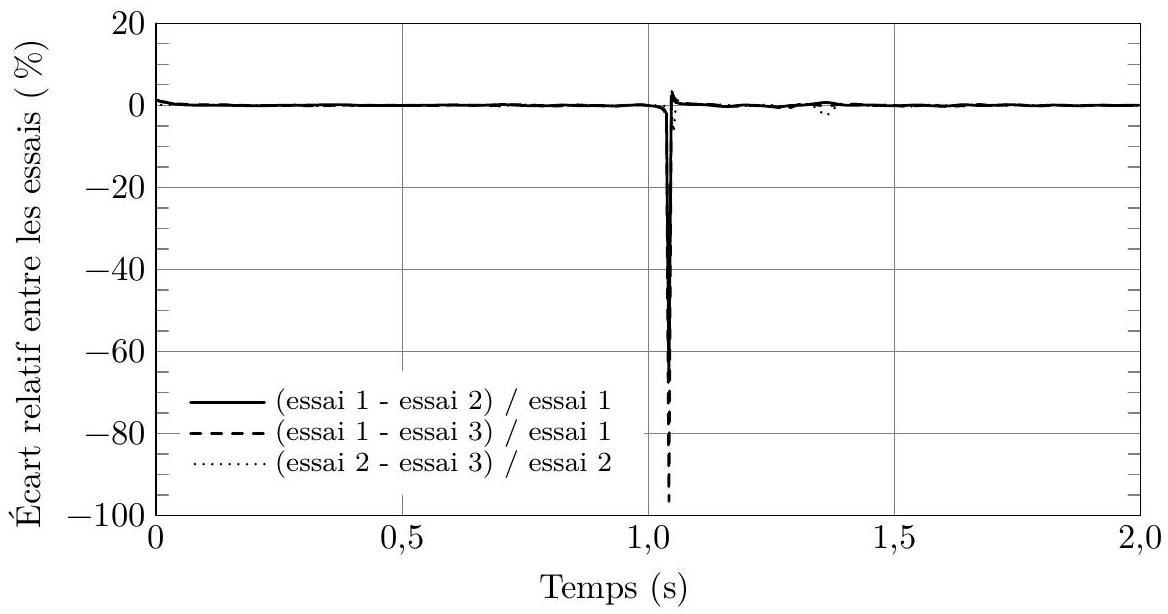
\includegraphics[width=\textwidth]{2025_07_06_ec63d2f3afc18cdeeb83g-12(1)}
%Figure 17 
\caption{\label{ccs_mp_2022_fig_17}Écarts expérimentaux relatifs entre les 3 essais}
\end{figure}



La durée totale de l'essai, accélération puis décélération, est de 2 secondes.\\
Prioritairement, les ingénieurs du bureau d'études veulent garantir :

\begin{itemize}
  \item la stabilité du système asservi, exigence Id = 1.1.1.1 ;
  \item la robustesse, exigence $\mathrm{Id}=1.1 .1 .3$.
\end{itemize}

Pour s'affranchir de la discontinuité en accélération, les ingénieurs du bureau d'études se limitent à l'étude en régime établi en négligeant la phase de transition entre l'accélération et la décélération autour de 1 seconde.
\fi

%Q 44. 
\question{\label{ccs_mp_2022_sec_q_44}Reproduire sur un croquis une des courbes de la figure \ref{ccs_mp_2022_fig_16} pour l'intervalle de temps $[0 \mathrm{~s}, 1 \mathrm{~s}]$. En s'appuyant sur ce croquis et une analyse chiffrée, indiquer si l'exigence $\mathrm{Id}=1.1 .1 .1 .2$ est atteinte.}
\ifprof
\begin{corrige}
%\begin{center}
%	\begin{tikzpicture}
%	\coordinate (O) at (0,0);
%	\def \myomega{2}
%	\def \myxf{10}
%	\def \myyf{4.5}
%	\def \myK{2.94}
%	\def \mytz{0}
%	\def\myT{2}
%	\def\myksii{.24}
%	\def\l{.2}
%	\def\mysmax{\myK*(1+exp(-pi*\myksii/sqrt(1-\myksii^2)))}
%	\def\myTp{2*pi/(\myomega*sqrt(1-\myksii^2))}
%	\def\tmax{\mytz + pi/(\myomega*sqrt(1-\myksii^2))}
%		\draw [->,>=latex] ($(O)+(-.5,0)$) -- node[pos=1,anchor=west] {$t$ [s]} ($(O)+(\myxf+.5,0)$) ;
%		\draw [->,>=latex] ($(O)+(0,-.5)$) -- node[pos=1,anchor=south, blue] {$\ddot x \text{ [m.s$^{-2}$]}$} ($(O)+(0,\myyf)$) ;
%		\draw[black] (\mytz,-.1) -- node[pos=0,anchor=north east] {$0$} (\mytz,.1);
%		\draw[black] (-.1,\myK) -- node[pos=0,anchor=east] {$2.94$} (.1,\myK);
%		\draw[black, dashed] (0,\myK) -- (\myxf-.5,\myK);
%		\draw[black] (-.1,{\mysmax}) -- node[pos=0,anchor=east] {$4$} (.1,{\mysmax});
%		\draw[black,dashed] (0,{\mysmax}) -- (4,{\mysmax}) ;
%	\draw[blue, thick, domain=\mytz:\myxf-.5, samples=150] 	plot	
%(\x,{\myK*(1-((exp(-\myomega*\myksii*(\x-\mytz))/sqrt(1-\myksii^2))*sin((180/pi)*\myomega*sqrt(1-\myksii^2)*(\x-\mytz)+atan(sqrt(1-\myksii^2)/\myksii))))});
%		\draw[<->,>=latex] ({\tmax},1) -- node[anchor=north] {$T_n$} ++  ({\myTp},0);
%		\draw[dashed] ({\tmax},1) --++ (0,3);
%		\draw[dashed] ({\tmax+\myTp},1) --++ (0,2.5);
%		\draw[black] (\myxf,-.1) -- node[pos=0,anchor=north east] {$1$} (\myxf,.1);
%	\end{tikzpicture}
%\end{center}

On a alors un dépassement de $\dfrac{4 - 2.94}{2.94} \simeq 0.36 \quad \text{soit 36\%} > 20\%$. L'exigence \texttt{Id : 1.1.1.1.2} n'est donc pas respectée.
\end{corrige}
\else
\fi

%Q 45. 
\question{\label{ccs_mp_2022_sec_q_45}À partir de la figure \ref{ccs_mp_2022_fig_17}, montrer de façon chiffrée que l'exigence Id $=1.1 .1 .3 .1$ est atteinte pour les conditions d'essais et d'interprétation fixées.}
\ifprof
\begin{corrige}
On peut observer en \textsc{Figure} \ref{fig:sled16} après une seconde, que l'écart relatif entre deux essais dépasse les $5\%$. L'exigence \texttt{Id : 1.1.1.3.1} n'est donc pas respectée.
\end{corrige}
\else
\fi

%IV.C - 
\subsection{Évolutions du modèle multiphysique \label{ccs_mp_2022_sec_4C}}
\begin{obj}
%\section*{Objectif}
L'objectif recherché par les ingénieurs du bureau d'études est à présent d'affiner les performances du modèle multiphysique et du dispositif expérimental (ou prototype) du Sled $0,3 g$.
\end{obj}

\ifprof
\else

La confrontation des performances expérimentales, avec celles obtenues en simulation avec le modèle $\mathrm{n}^{\circ} 1$ (figure \ref{ccs_mp_2022_fig_20}), permet d'affirmer que le modèle $n^{\circ} 1$ n'est pas totalement représentatif du comportement réel du prototype du Sled. Un modèle multiphysique $\mathrm{n}^{\circ} 2$ (figure \ref{ccs_mp_2022_fig_21}) est développé. Il comporte désormais à la fois
la correction PI précédemment définie, mais aussi une prise en compte plus réaliste de la partie mécanique précédemment décrite.

Le résultat de la simulation de ce modèle $\mathrm{n}^{\circ} 2$ (figure \ref{ccs_mp_2022_fig_21}) à une consigne d'accélération en échelon de $0,3 g$ est présenté sur la figure \ref{ccs_mp_2022_fig_18}. Le résultat expérimental du prototype du Sled est également représenté sur cette figure et peut ainsi être comparé. Le résultat de la simulation du modèle $\mathrm{n}^{\circ} 1$ avec correction proportionnelle intégrale y est également rappelé. Les trois courbes correspondent à une même masse embarquée de 80 kg .

\begin{figure}[!h]
\centering

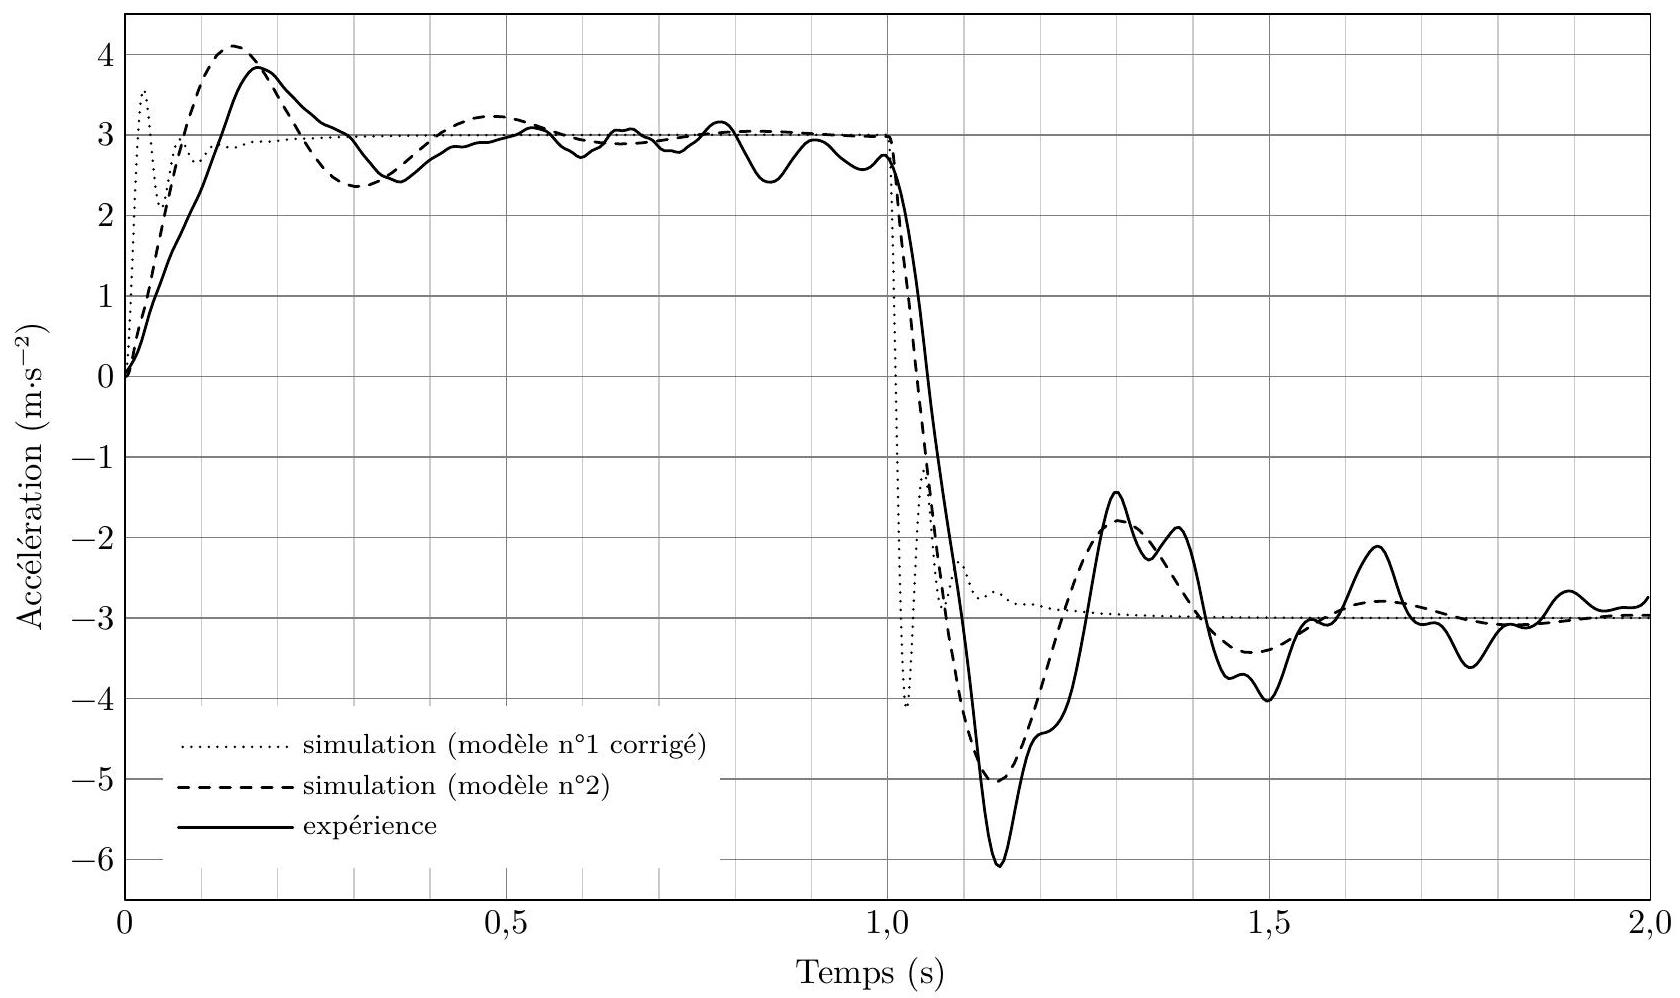
\includegraphics[width=\textwidth]{2025_07_06_ec63d2f3afc18cdeeb83g-13}

%Figure 18 
\caption{\label{ccs_mp_2022_fig_18}Comparaison des résultats expérimentaux sur le prototype du Sled avec ceux issus des deux simulations. }
Légende :

\begin{itemize}
  \item << expérience >>, résultats expérimentaux obtenus avec le Sled;
  \item << simulation (modèle $\mathrm{n}^{\circ} 2$ ) >>, le modèle $\mathrm{n}^{\circ} 2$ comportant la correction PI comme défini en figure \ref{ccs_mp_2022_fig_21} ;
  \item << simulation (modèle $\mathrm{n}^{\circ} 1$ corrigé) >>, modèle $\mathrm{n}^{\circ} 1$ défini en figure \ref{ccs_mp_2022_fig_20} avec ajout d'une correction PI définie à partir de la figure \ref{ccs_mp_2022_fig_10}.
\end{itemize}
\end{figure}


Il apparait que la courbe << simulation (modèle $\mathrm{n}^{\circ} 2$ ) >> est plus proche de la courbe << expérience >> que la courbe intitulée << simulation (modèle $\mathrm{n}^{\circ} 1$ corrigé) >>. Elle présente plus de dépassements et d'oscillations. Le second modèle présenté en figure \ref{ccs_mp_2022_fig_21} est donc plus proche de la réalité du prototype du Sled $0,3 g$ que le modèle multiphysique $\mathrm{n}^{\circ} 1$ (figure \ref{ccs_mp_2022_fig_20}) avec correction (figure \ref{ccs_mp_2022_fig_10}).

Dans cette comparaison, l'apport du modèle multiphysique $n^{\circ} 2$ se situe principalement sur l'ajout de la zone entourée d'un ovale en figure \ref{ccs_mp_2022_fig_21}.
\fi


%Q 46. 
\question{\label{ccs_mp_2022_sec_q_46}Préciser quel composant technologique du prototype du Sled est modélisé par la zone entourée d'un ovale en figure \ref{ccs_mp_2022_fig_21} et qui permet de diminuer l'écart entre le résultat de la «simulation (modèle $\mathrm{n}^{\circ} 2$ ) » et le comportement expérimental.}
\ifprof
\begin{corrige}
Le composant technologique modélisé par la zone entourée d'un ovale est la courroie C2.
\end{corrige}
\else
\fi

%V
\section{Synthèse des performances réalisées par le modèle multiphysique $\mathrm{n}^{\circ} 2$ et évolution du prototype (ou dispositif expérimental) du Sled $0,3 g$ \label{ccs_mp_2022_sec_5}}

L'objectif est à présent de fournir aux ingénieurs une synthèse du travail réalisé et à poursuivre.

\ifprof
\else


Plusieurs simulations ont été réalisées avec le modèle multiphysique $\mathrm{n}^{\circ} 2$ pour différentes masses de passagers potentiellement embarqués de 30 à 150 kg . Les résultats sont présentés en figure \ref{ccs_mp_2022_fig_19}. Seule la première partie de la courbe de simulation d'un cycle complet est représentée. Elle correspond à une accélération constante $a_{c}=+0,3 g$ pendant 1 seconde.

\begin{figure}[!h]
\centering
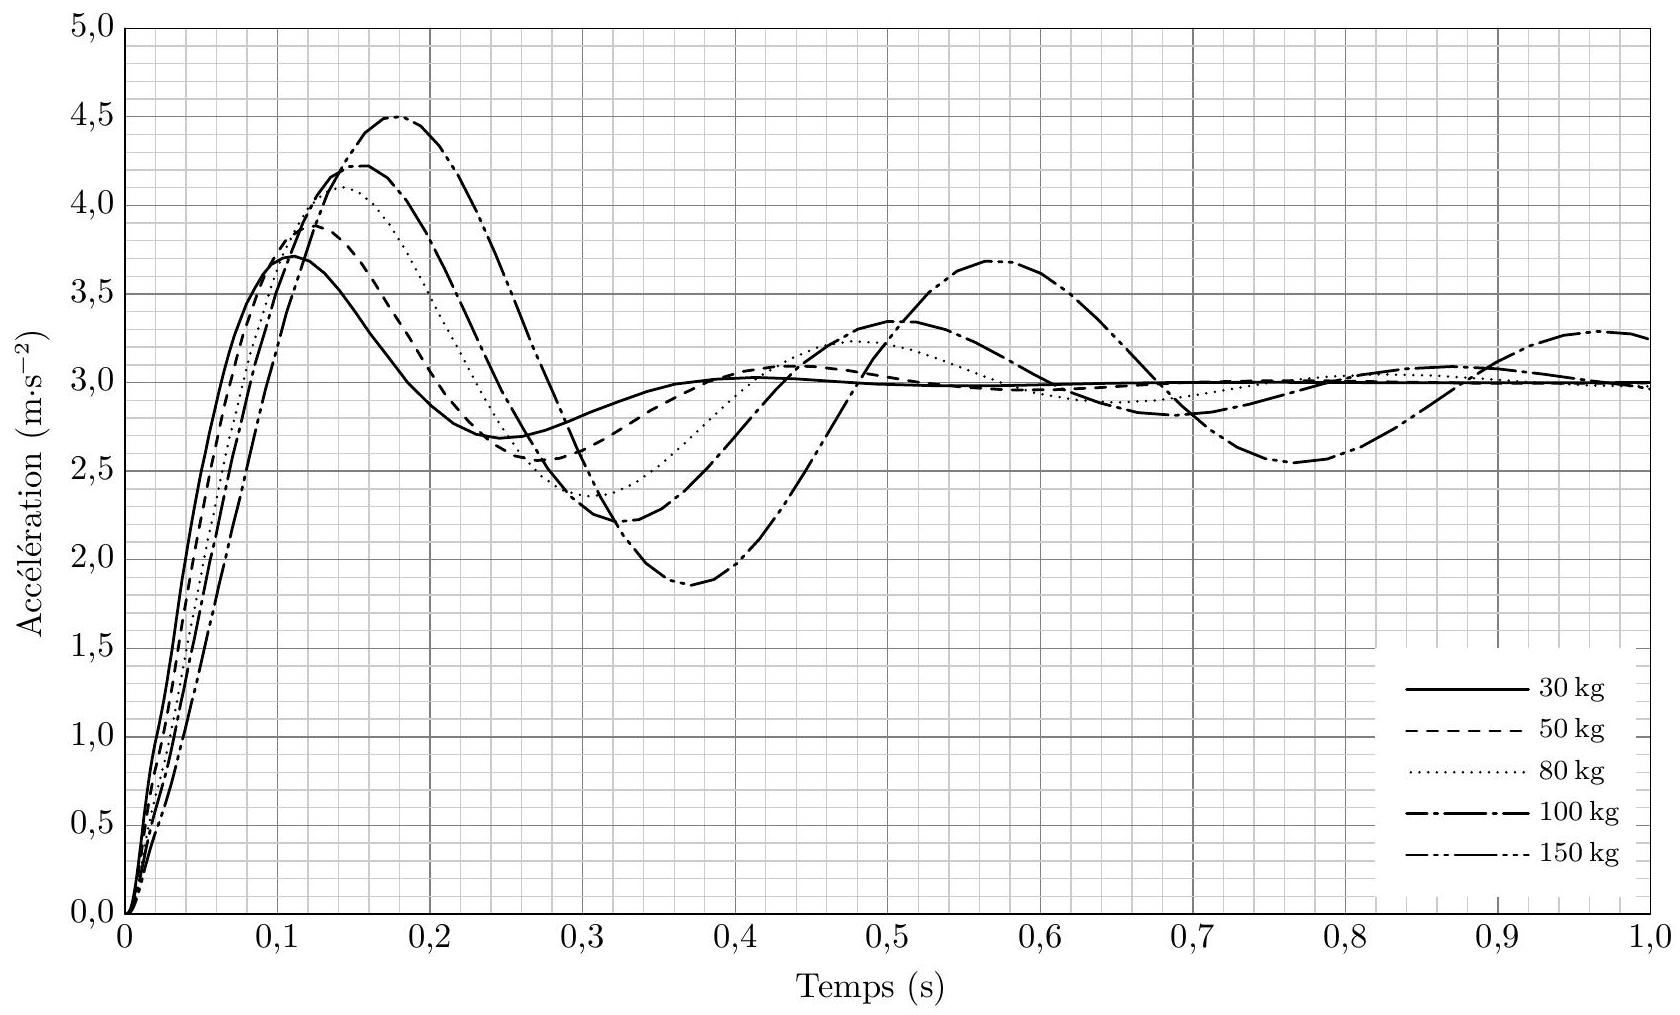
\includegraphics[width=\textwidth]{2025_07_06_ec63d2f3afc18cdeeb83g-14}

%Figure 19 
\caption{\label{ccs_mp_2022_fig_19}Simulations du modèle multiphysique $n^{\circ} 2$ pour différentes masses de passagers}
\end{figure}
\fi

%Q 47. 
\question{\label{ccs_mp_2022_sec_q_47}À partir de la figure \ref{ccs_mp_2022_fig_19}, parmi les exigences vérifiables, identifier et lister celles qui ne sont pas validées. Préciser, pour chacune d'elles, à partir de quelle valeur de masse ces exigences ne sont plus vérifiées.}
\ifprof
\begin{corrige}
\begin{itemize}
\item \texttt{Id : 1.1.1.1.1} : $M G < 7$ dB et $M P > 30\degres$. Cette exigence ne peut pas être vérifiée à l'aide de la \textsc{Figure} \ref{fig:sled19}.\\

\item \texttt{Id : 1.1.1.1.2} : le premier dépassement doit être inférieur à $20\%$. On observe alors sur la \textsc{Figure} \ref{fig:sled19} :

	\begin{itemize}
	\item $30$ kg : $\dfrac{3.7-2.94}{2.94} \simeq 26\%$\\
	\end{itemize}

le premier dépassement de $30$ kg étant le plus faible, l'exigence n'est donc pas validée.\\

\item \texttt{Id : 1.1.1.2.1} : la précision doit être inférieure à $10\%$ en régime permanent :

	\begin{itemize}
	\item $150$ kg : $\dfrac{3.3-2.94}{2.94} \simeq 12\%$

	\item $100$ kg : $\dfrac{3.1-2.94}{2.94} \simeq 5.4\%$\\
	\end{itemize}

la précision augmentant avec la diminution du poids, l'exigence est validée pour les poids inférieurs ou égaux à $100$ kg.\\
 
\item \texttt{Id : 1.1.1.3.1} : l'écart relatif entre deux essais doit être inférieur à $\pm5\%$. Cette exigence ne peut pas être vérifiée à l'aide de la \textsc{Figure} \ref{fig:sled19}.\\

\item \texttt{Id : 1.1.1.4.1} : le temps de réponse à $5$\% doit être inférieur à $0.25$ s. En observant les différentes réponses temporelles de la \textsc{Figure} \ref{fig:sled19}., on remarque qu'à $0.25$ s, aucun des signaux ne respecte l'exigence.
\end{itemize}

\end{corrige}
\else
\fi

\ifprof
\else
Afin de gérer l'avancement du projet de recherche, le bureau d'études a développé un graphe d'états applicable aussi bien au dimensionnement et à la réalisation du Sled $0,3 g$ qu'à celui du Sled $1 g$ (figure \ref{ccs_mp_2022_fig_B} du document réponse).
\fi

%Q 48. 
\question{\label{ccs_mp_2022_sec_q_48}Retracer le parcours effectué dans cette démarche de conception en repassant en couleur, sur la figure \ref{ccs_mp_2022_fig_B}, les liens concernés et entourer la situation dans laquelle se trouve l'avancement actuel du projet de Sled $0,3 g$.}
\ifprof
\begin{corrige}
\end{corrige}
\else
\fi

\ifprof
\else

\begin{figure}[!h]
\centering

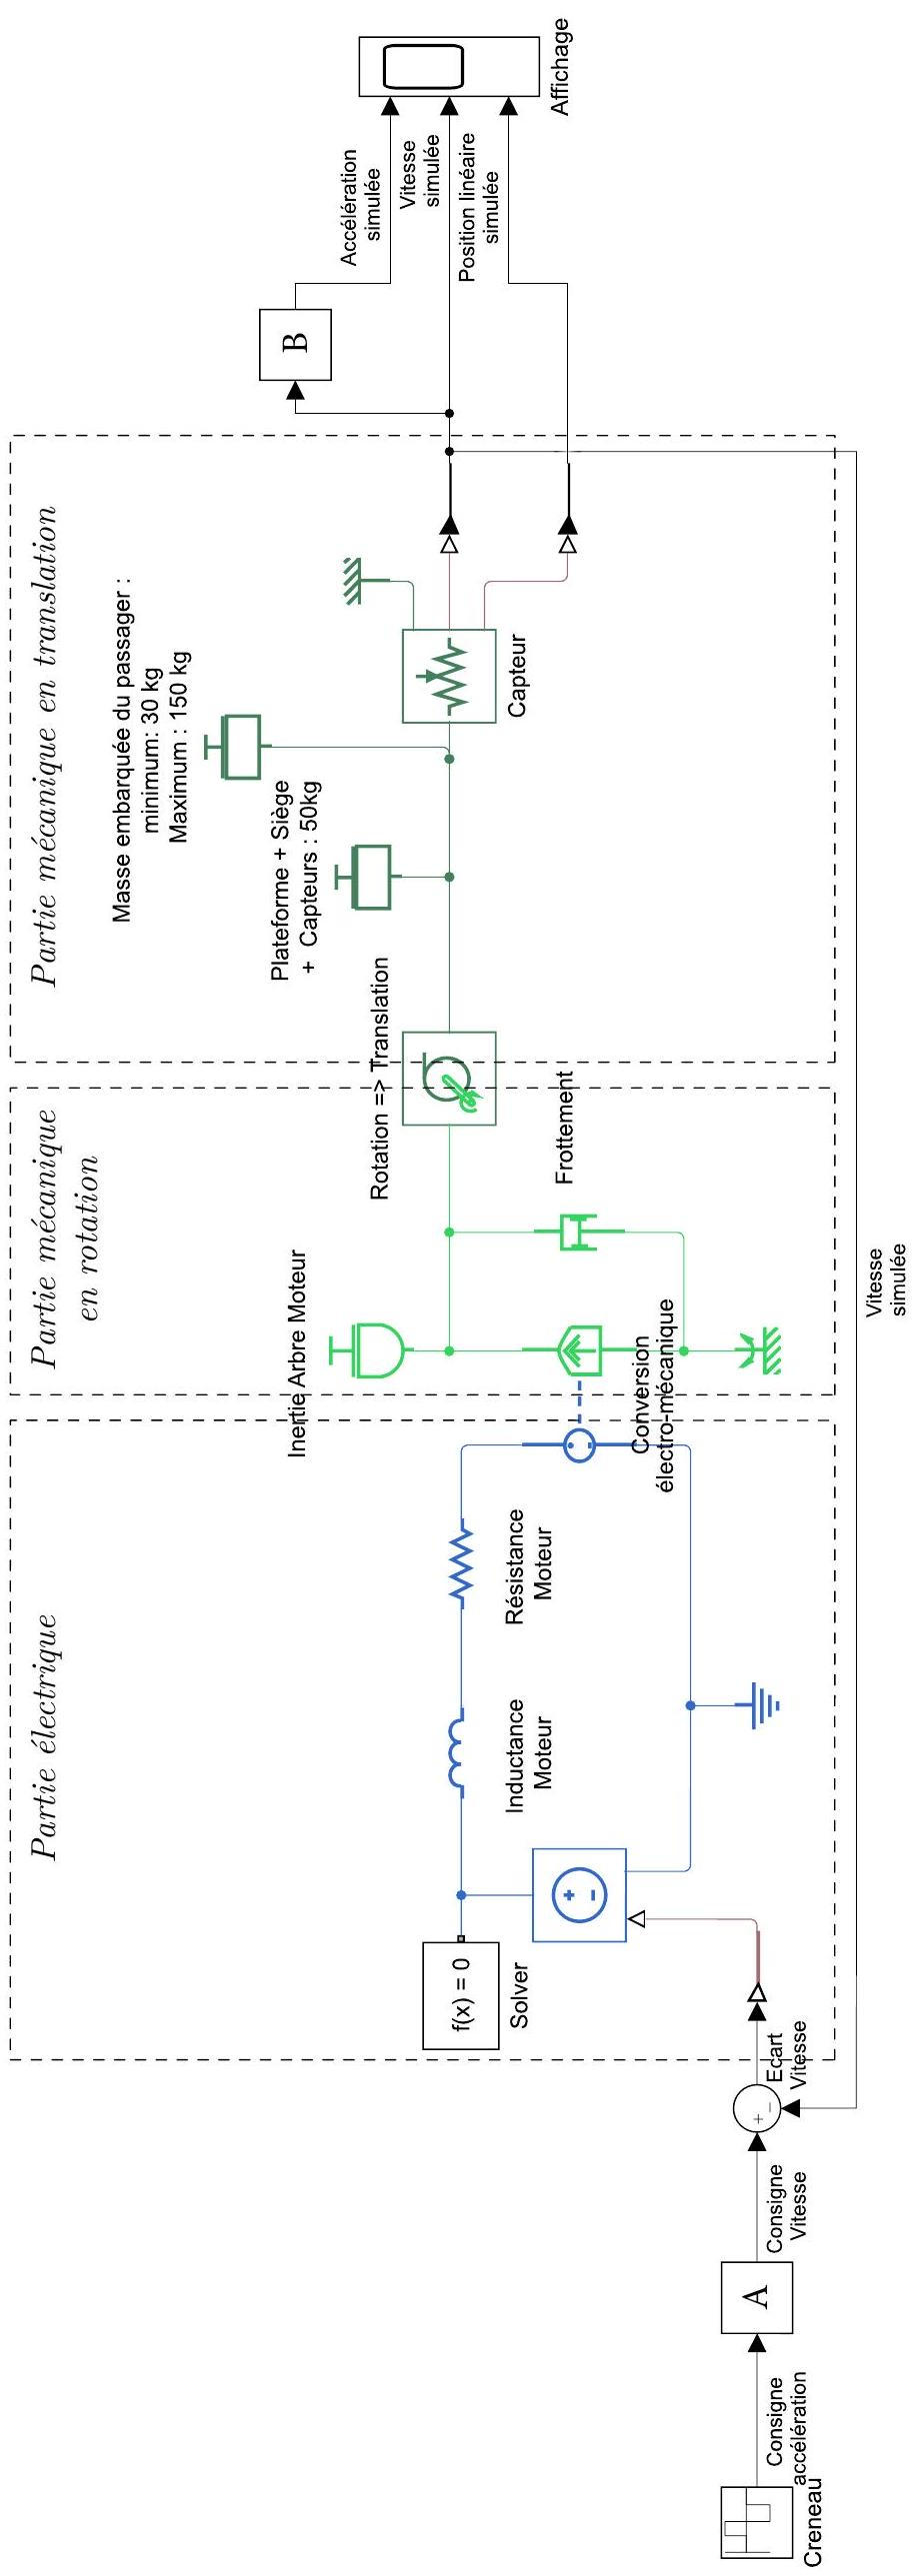
\includegraphics[height=.95\textheight]{2025_07_06_ec63d2f3afc18cdeeb83g-15}
%Figure 20 
\caption{\label{ccs_mp_2022_fig_20}Modèle $n^{\circ} 1$ du Sled}
\end{figure}


\begin{figure}[!h]
\centering
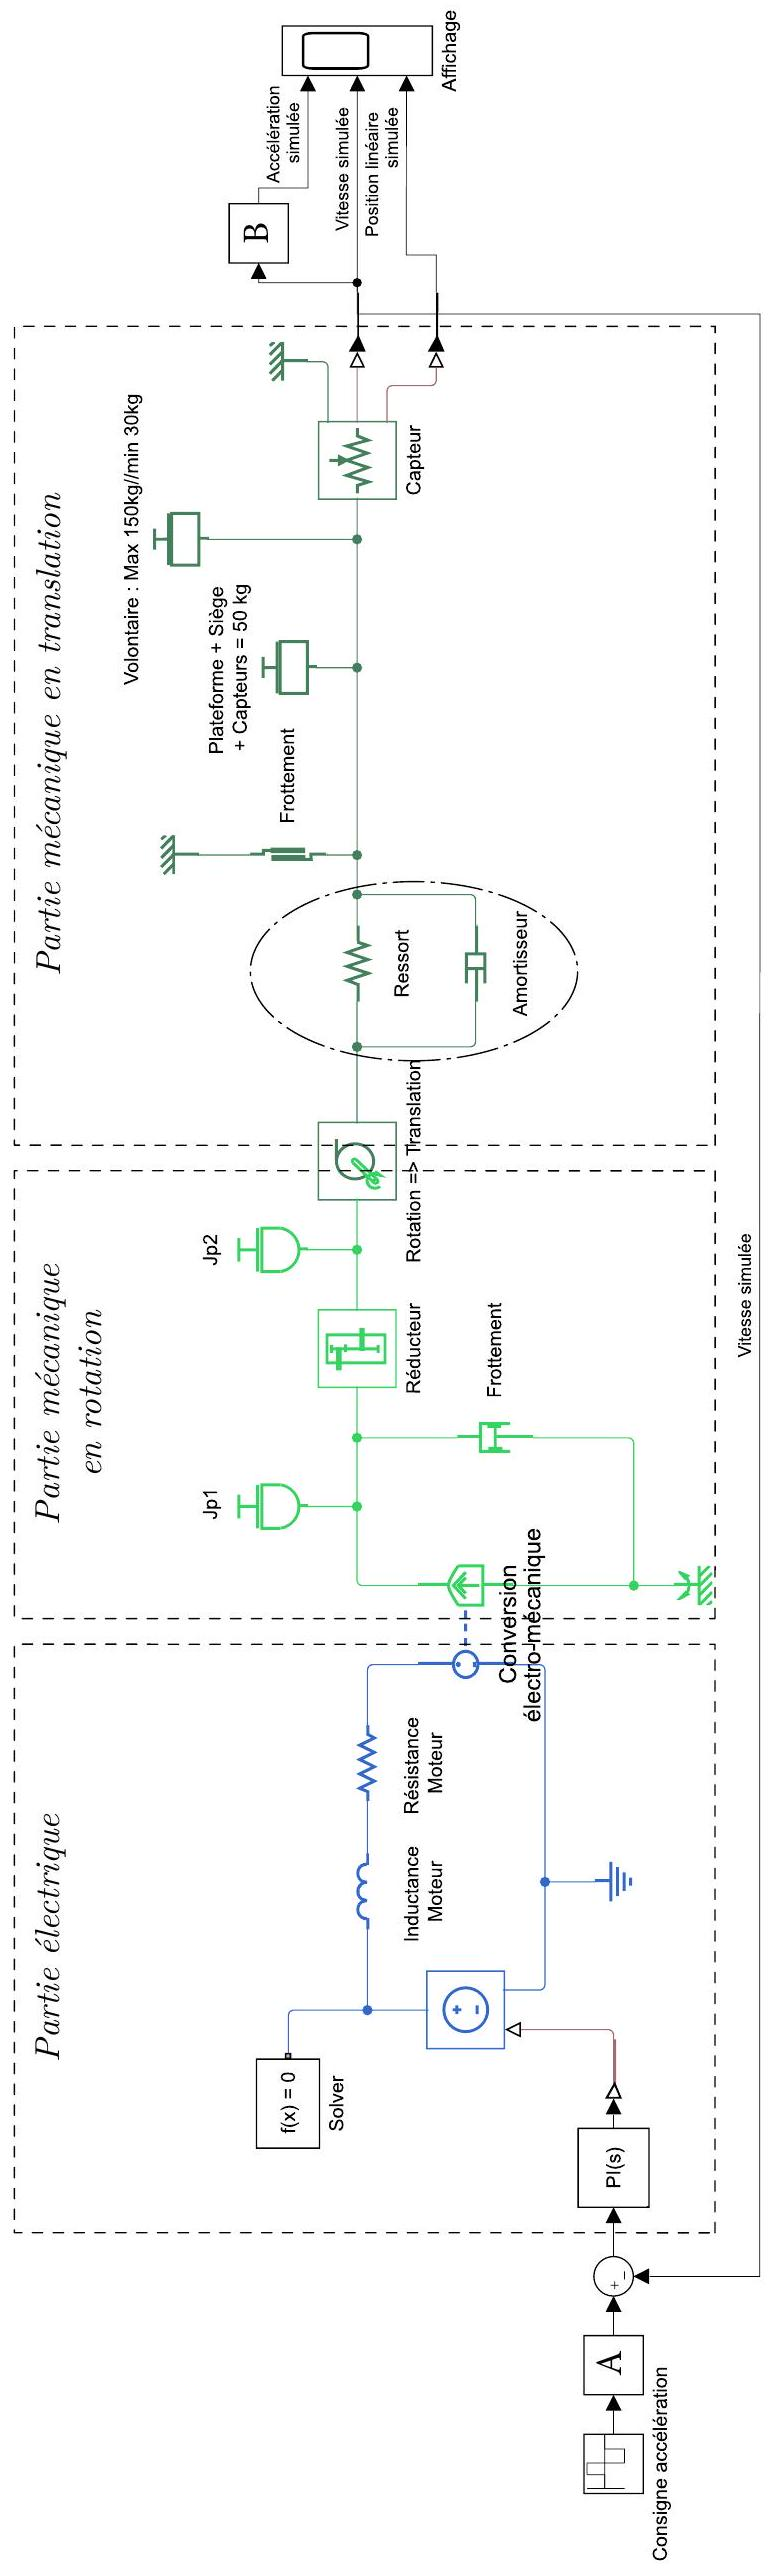
\includegraphics[height=.9\textheight]{2025_07_06_ec63d2f3afc18cdeeb83g-16}

%Figure 21 
\caption{\label{ccs_mp_2022_fig_21}Modèle multiphysique $\mathrm{n}^{\circ} 2$}
\end{figure}

\fi



\ifprof
\else
Document réponse pour l'épreuve de S2I\\

\begin{figure}[!h]
\centering
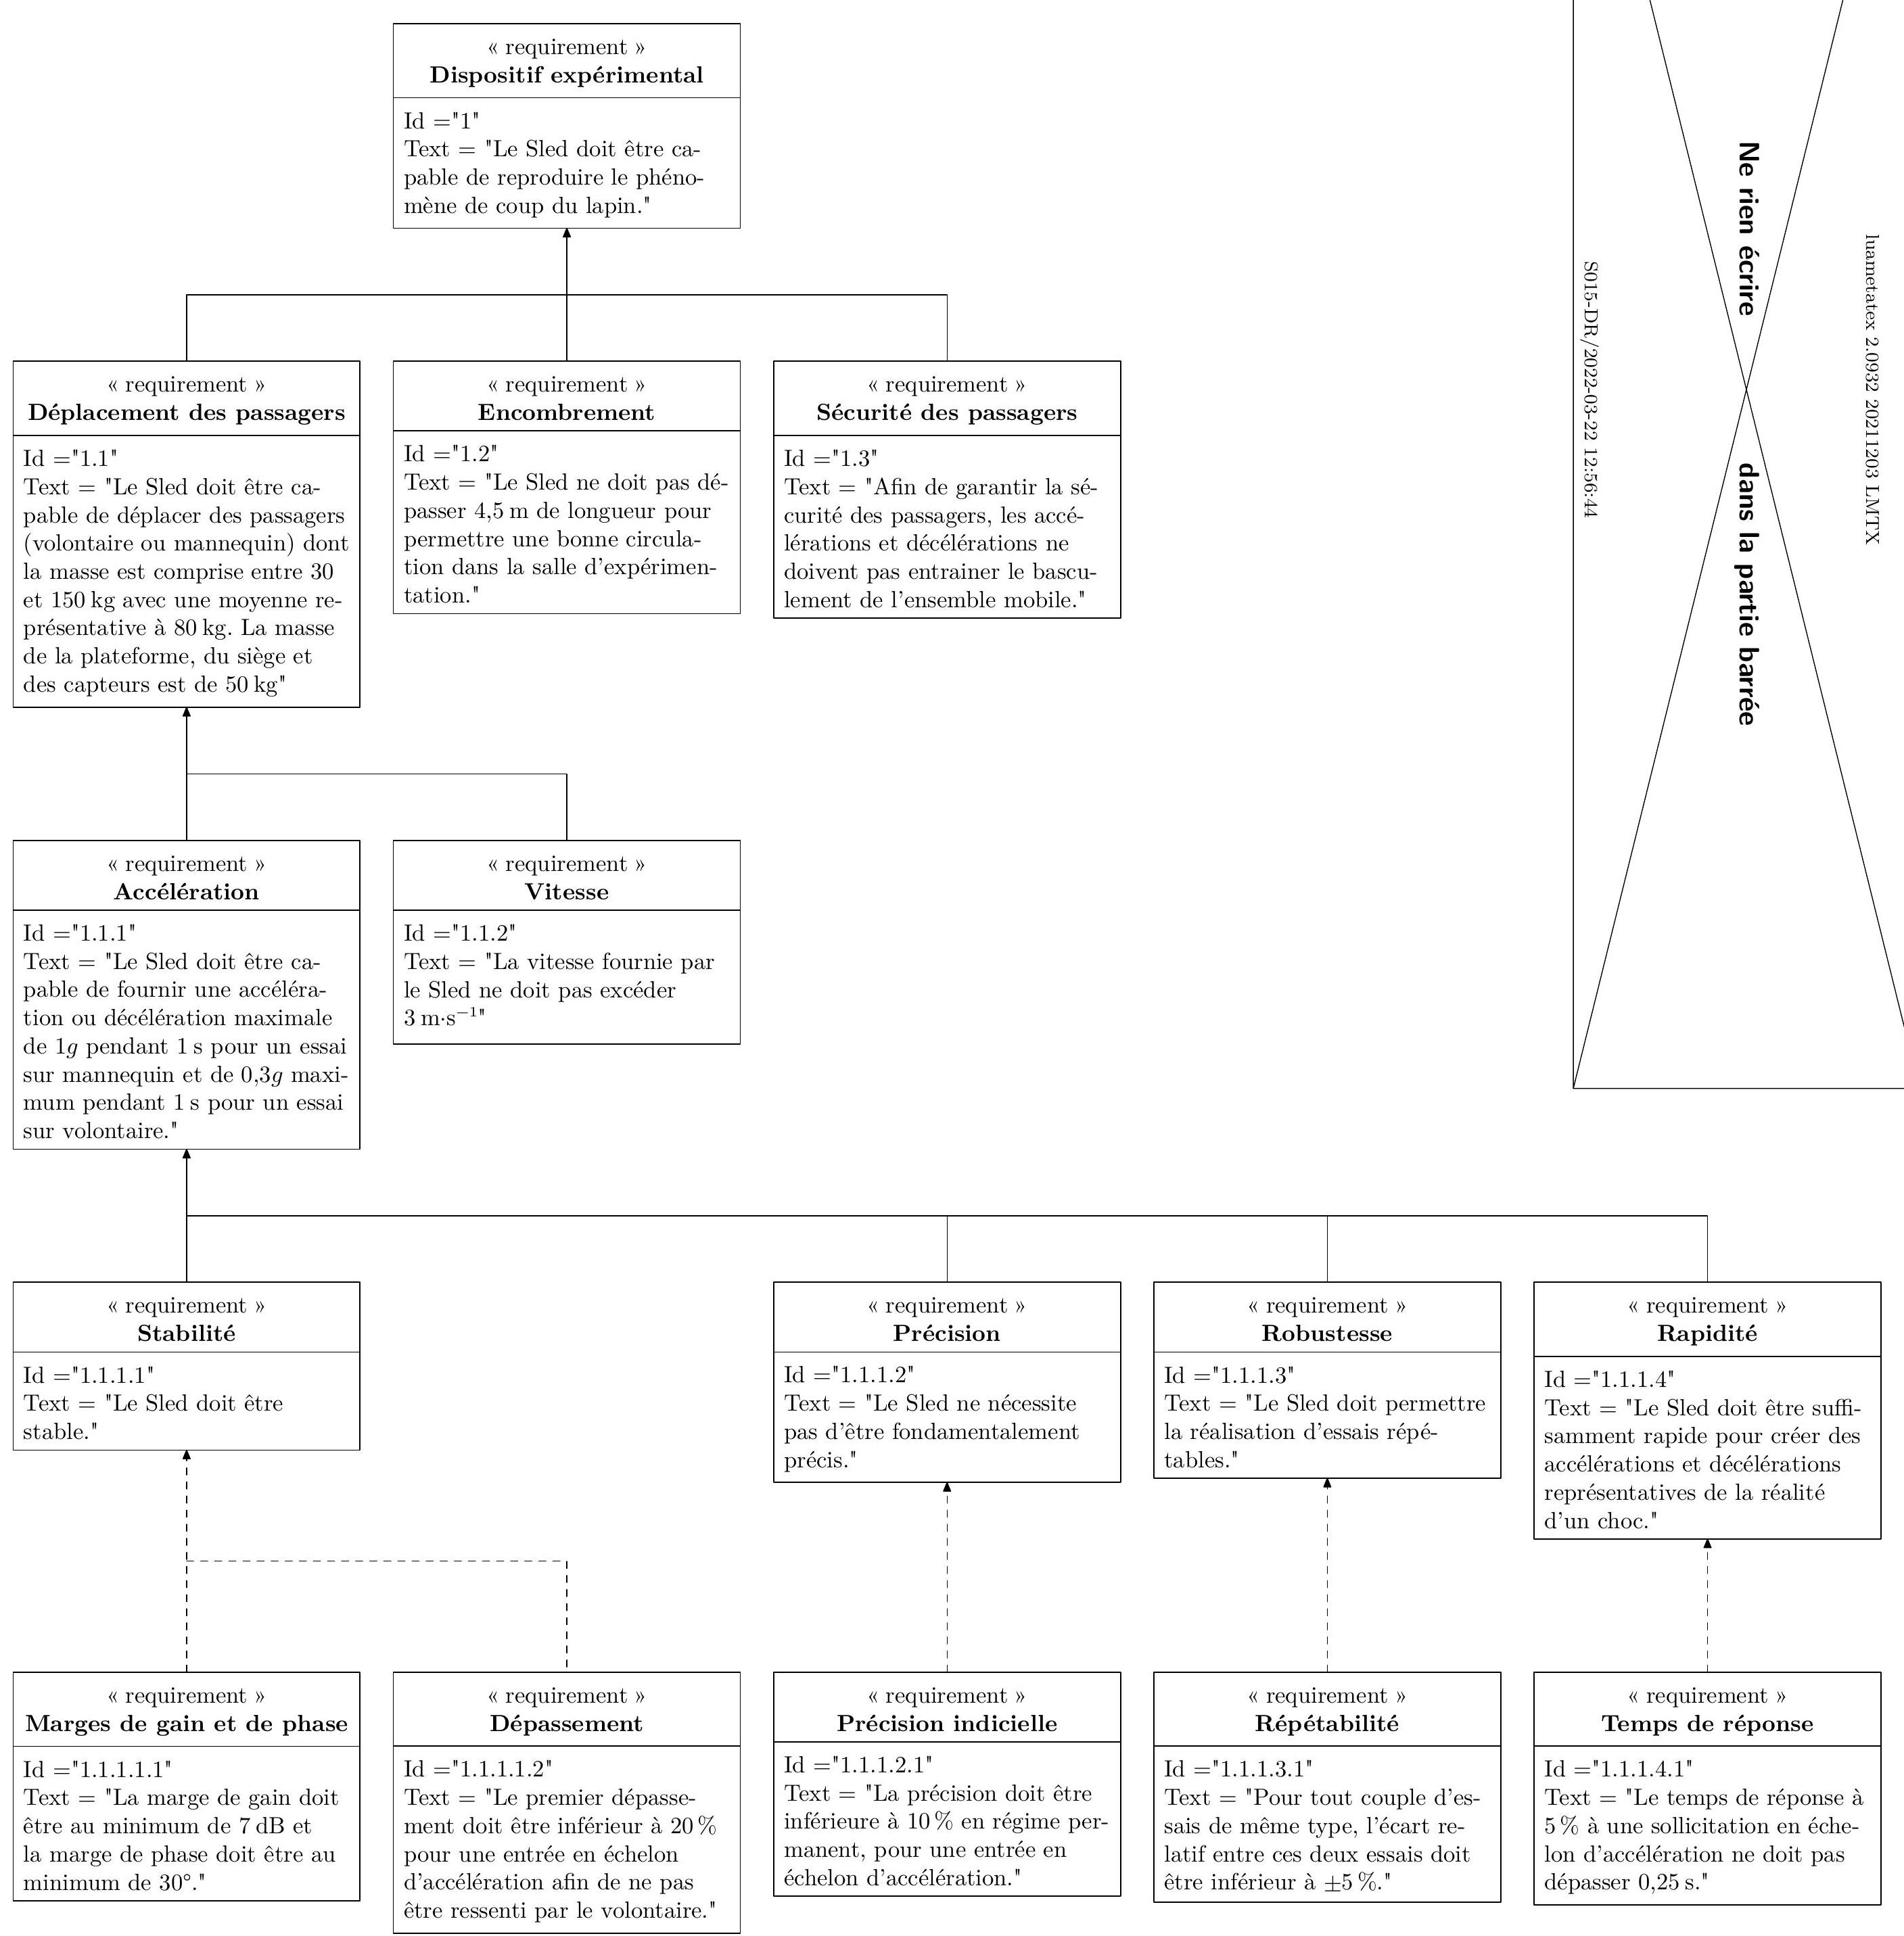
\includegraphics[width=\textwidth]{2025_07_06_ec63d2f3afc18cdeeb83g-18}

%Figure A 
\caption{\label{ccs_mp_2022_fig_A}Diagramme partiel des exigences du Sled}
\end{figure}

\section*{Question 48}
\begin{figure}[!h]
\centering

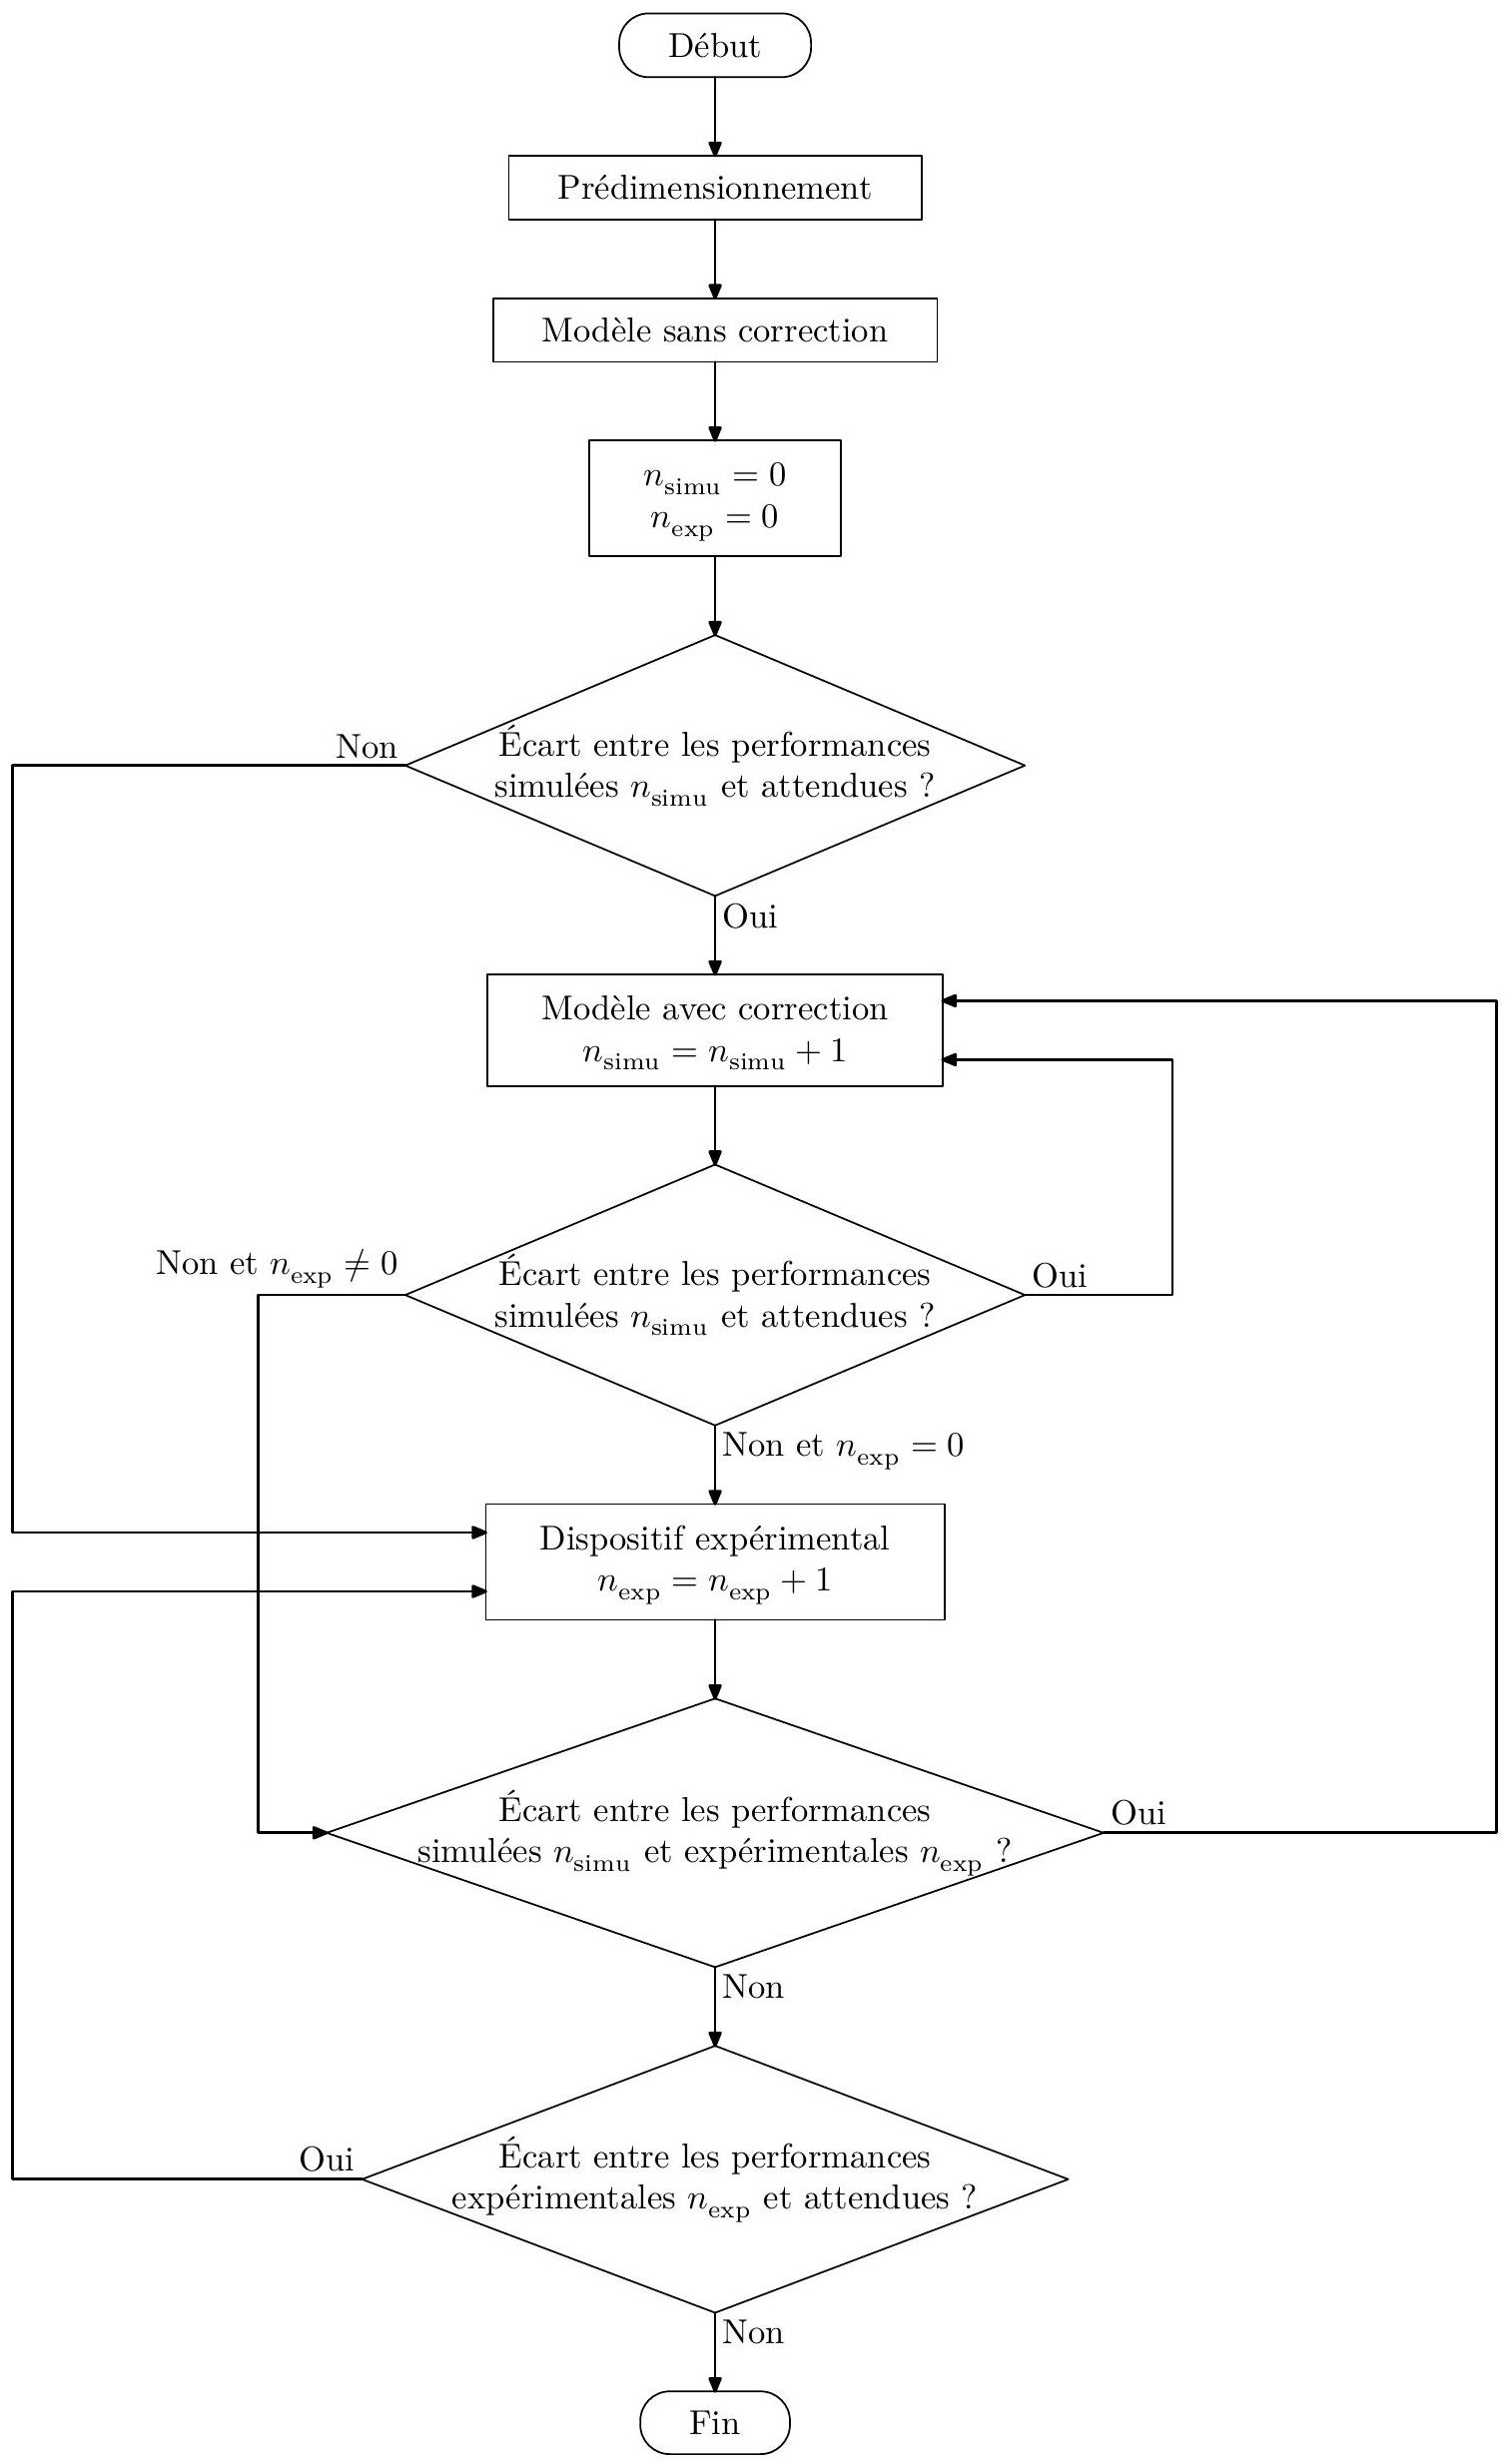
\includegraphics[max width=.8\textwidth]{2025_07_06_ec63d2f3afc18cdeeb83g-19}

%Figure B 
\caption{\label{ccs_mp_2022_fig_B}Graphe d'états du projet de développement du Sled}
\end{figure}

\fi
